% Place an \includeonly here to only compile certain parts
% e.g.: \includeonly{title,chapter-first,references}

\documentclass[12pt,oneside]{book}
\usepackage[T1]{fontenc}
\usepackage{fancyhdr}           % For page number in the upper right
                                % (required) and other running headers
                                % (optional)
\usepackage{setspace}           % For double-spacing (required)
\usepackage{titlesec}           % For keeping section/chapter titles
                                % single-spaced
\usepackage{etoolbox}           % For the flag determining if front matter
                                % goes into the TOC
\usepackage{blindtext}          % For generating dummy text in the sample
\usepackage{amsmath,graphicx,multirow,diagbox,amssymb,extpfeil,color,epstopdf}
%\usepackage{natbib}
\usepackage{subcaption}
\usepackage{graphicx,adjustbox,pdflscape,tabu,diagbox,algorithm2e}

\SetKwInOut{Parameter}{parameter}
\newcommand{\tabitem}{~~\llap{\textbullet}~~}



\DeclareMathOperator*{\argmin}{argmin}
% Header height (to avoid fancyhdr error)
\setlength{\headheight}{13.6pt}

% Header formatting for regular pages
\fancyhf{}
\fancyhead[L]{\it\small\leftmark}
\fancyhead[R]{\small\thepage}

% Header formatting for chapter title pages
\fancypagestyle{plain}{%
  \fancyhf{}
  \fancyhead[R]{\small\thepage}
  \renewcommand{\headrulewidth}{0pt}
}

% Formatting of chapter and section titles: keep them single-spaced in the
% midst of double-spaced text
\titleformat{\chapter}[display]%
{\bfseries\singlespacing\Large}%
{Chapter~\thechapter}%
{1em}%
{\LARGE}

\titleformat{\section}[hang]%
{\bfseries\singlespacing\Large}%
{\thesection}%
{0.25in}%
{}

\titleformat{\subsection}[hang]%
{\bfseries\singlespacing\large}%
{\thesubsection}%
{0.25in}%
{}

% Flag for whether to add front matter to TOC
\newtoggle{fulltoc}
\togglefalse{fulltoc}  % Change to \toggletrue{fulltoc} to include front matter

\begin{document}

% Title page
% TITLE PAGE

% Sample text taken from the June 2014 version of "Preparing Your Thesis" by
% the Office of the University Dean of Graduate Studies at the University of
% Rochester

\begin{titlepage}
  \vspace*{\fill}

  \begin{center}
    {\LARGE \bfseries Dissertation Title Typed in Upper and Lower Case
      Letters \par
    }

    \bigskip%
    by

    \bigskip%
    Your Name [no degree credentials]

    %%%%%

    \bigskip\bigskip\bigskip\bigskip%
    Submitted in Partial Fulfillment of the

    \bigskip%
    Requirements for the Degree

    \bigskip%
    Doctor of Philosophy

    %%%%%

    \bigskip\bigskip\bigskip\bigskip%
    Supervised by Professor [Your advisor's first and last name]

    \bigskip\bigskip%
    [Department if applicable]

    \bigskip%
    [School Name 1]

    \bigskip%
    [School Name 2]

    %%%%%

    \bigskip\bigskip\bigskip\bigskip%
    University of Rochester

    \bigskip%
    Rochester, New York

    %%%%%

    \bigskip\bigskip\bigskip\bigskip%
    2014 [or year of degree conferral]
  \end{center}

  \vspace*{\fill}
\end{titlepage}

%%% Local Variables:
%%% mode: latex
%%% TeX-master: "dissertation"
%%% End:


% All subsequent pages must be numbered, title page is considered page i,
% front matter is numbered in lowercase Roman numerals
\pagestyle{fancy}
\pagenumbering{roman}
\setcounter{page}{2}
\doublespacing

% Dedication (optional)
% DEDICATION

\thispagestyle{plain}

\begin{center}
  \vspace*{\fill}

  \it%
  Dedication goes here.

  \vspace*{\fill}
\end{center}

\clearpage

%%% Local Variables: 
%%% mode: latex
%%% TeX-master: "dissertation"
%%% End: 


% Biographical sketch
% BIOGRAPHICAL SKETCH

% Sample text taken from the June 2014 version of "Preparing Your Thesis" by
% the Office of the University Dean of Graduate Studies at the University of
% Rochester

\chapter*{Biographical Sketch}
\markboth{\MakeUppercase{Biographical Sketch}}{}
\iftoggle{fulltoc}{
  \addcontentsline{toc}{chapter}{Biographical Sketch}
}{}

The author was born in CITY, STATE. HE/SHE attended XXXX University, and
graduated with a Bachelor of ARTS/SCIENCE degree in MAJOR FIELD. Describe
Master's degree if from an institution other than the University of
Rochester. Describe professional or career path prior to doctoral study if
applicable. HE/SHE began doctoral studies in FIELD at the University of
Rochester in 200X. HE/SHE was awarded [if applicable: a NAME(s) Fellowship in
200X and 200X] and [if applicable] received the Master of ARTS/SCIENCE degree
from the University of Rochester. HE/SHE pursued HIS/HER research in SUBJECT
under the direction of ADVISOR NAME.

\bigskip\noindent%
The following publications were a result of work conducted during doctoral
study: [list full bibliographic reference information in the format used
elsewhere in the dissertation]

%%% Local Variables: 
%%% mode: latex
%%% TeX-master: "dissertation"
%%% End: 


% Acknowledgments
\include{04-acknowledgments}

% Abstract
% ABSTRACT

\chapter*{Abstract}
\markboth{\MakeUppercase{Abstract}}{}
\iftoggle{fulltoc}{
  \addcontentsline{toc}{chapter}{Abstract}
}{}

\Blindtext[3]

%%% Local Variables: 
%%% mode: latex
%%% TeX-master: "dissertation"
%%% End: 


% Contributors and Funding Sources
% CONTRIBUTORS AND FUNDING SOURCES

% Sample text taken from the June 2014 version of "Preparing Your Thesis" by
% the Office of the University Dean of Graduate Studies at the University of
% Rochester

\chapter*{Contributors and Funding Sources}
\markboth{\MakeUppercase{Contributors and Funding Sources}}{}
\iftoggle{fulltoc}{
  \addcontentsline{toc}{chapter}{Contributors and Funding Sources}
}{}

This work was supported by a dissertation committee consisting of Professor
XXXX (advisor --- also note if co-advisor) and XXXX of the Department of (Home
Department) and Professor(s) XXXX of the Department of (Outside
Department). The data analyzed for Chapter 3 was provided by Professor
XXXX. The analyses depicted in Chapter 4 were conducted in part by Rebecca
Jones of the Department of Biostatistics and were published in (year) in an
article listed in the Biographical Sketch. All other work conducted for the
dissertation was completed by the student independently. (If applicable)
Graduate study was supported by a Provost Fellowship from the University of
Rochester and a dissertation research fellowship from XXX Foundation.


%%% Local Variables: 
%%% mode: latex
%%% TeX-master: "dissertation"
%%% End: 


% Table of Contents, List of Tables, List of Figures
% CONTENTS

% Main TOC
\tableofcontents

% List of tables, if applicable
\listoftables
\iftoggle{fulltoc}{
  \addcontentsline{toc}{chapter}{List of Tables}
}{}

% List of figures, if applicable
\listoffigures
\iftoggle{fulltoc}{
  \addcontentsline{toc}{chapter}{List of Figures}
}{}


%%%%%%%%%%%%%%%%%%%% DISSERTATION CONTENT %%%%%%%%%%%%%%%%%%%%

% Regular numbering starts now, first page of first chapter is page 1
\clearpage
\setcounter{page}{0}
\pagenumbering{arabic}

% Body
\chapter{A Chapter with a Mathematical Appendix}
\label{cha:has-app}

\Blindtext[1]

\section{A Section}

\Blindtext[1]

\section{Another Section}

\Blindtext[1]

%%%%%%%%%% APPENDIX %%%%%%%%%%

% Redefine sectioning as letters
\setcounter{section}{0}
\let\oldthesection\thesection
\renewcommand{\thesection}{\thechapter.\Alph{section}}
\section{Appendix to Chapter~\ref{cha:has-app}}

Sometimes you might want a chapter-specific appendix numbered separately from
the section numbers in the main text.
This is especially useful when you are dealing with numbered equations or
theorems, and want a way to denote that a result lives in the appendix.
See the source code for this chapter for how this is done.

% Go back to the old section numbering for future chapters
\let\thesection\oldthesection

%%% Local Variables: 
%%% mode: latex
%%% TeX-master: "dissertation"
%%% End: 

\chapter{A Local-Linear-Fitting-Based Matting Approach for Accurate Depth Upsampling}
\label{cha2}
\chaptermark{Local-Linear-Fitting-Based Depth Upsampling}

\section{Introduction}
\label{sec:2.1.intro}
Depth upsampling aims at obtaining high resolution depth maps based on low resolution version. Naive method such as bilinear or bicubic interpolation uses only depth informations, which result in the problem of blurred, gradual-changing edges, making the interpolation terrible for complex scenes. To overcome this problem, color image can be exploited to constraint the interpolation consistent within contours. For smooth area, simple bilinear methods usually can provide a satisfying results and advanced algorithms can behave similar to keep the procedure compact. We obey this observation and provide a local linear fitting based matting approach for accurate depth spsampling in this chapter.

This chapter will discuss a local-linear-fitting based matting approach for accurate depth upsampling, and the memory saving optimization method using conjugate gradient solver. This chapter is organized as follows: Section~\ref{sec:2.relate_work} briefly discuss related literature to depth upsampling. Section~\ref{sec:2.algo} describes the scheme of our algorithm, and the memory saving solver. We present both the quantitative and the qualitative results in Section~\ref{sec:2.result}, and conclude the paper in Section~\ref{sec:2.conclusion}.

\section{Related work}
\label{sec:2.relate_work}
Traditionally depth upsampling is accomplished by bilinear or bicubic interpolation. These methods have difficulty in preserving the sharp edges in depth maps. Several methods have been developed to overcome these problems, aiming at improving the accuracy of depth upsampling problem. One class of techniques relies on proposing a prior and optimizing an objective function that combines prior and data fidelity terms~\cite{diebel2005application,yang2007spatial,he2010guided,kopf2007joint,park2011high,ferstl2013image,yang2014color}. 
Diebel and Thrun~\cite{diebel2005application} proposed an upsampling algorithm based on Markov random field (MRF), which is defined through depth measure potential, depth smooth prior and weighting factors. This MRF framework is further improved by other researchers, such as~\cite{lu2011revisit} and~\cite{harrison2010image}. Yang et al.~\cite{yang2007spatial} made use of a bilateral filter in an iterative refinement framework. The refinement is constructed on a cost volume defined on the current depth map and the RGB image. This algorithm can also work on two view depth map refinement with a different cost volume definition. In~\cite{he2010guided}, the guided filter was designed for edge preserving filter, which can be viewed as an extension of the bilateral filter. Kopf et al.~\cite{kopf2007joint} proposed joint a bilateral filter which is also similar in principle. Both filters can be used to upsample the depth map with a high resolution RGB image. Park et al.~\cite{park2011high} gave an algorithm based on a non local mean filter. The low resolution depth map is pre-processed to detect outliers. These points are removed and to obtain the high resolution depth map an objective function consisting of a smooth term, non-local structure term and data term is optimized. This algorithm is also suitable for filling large holes in the depth data. Ferstl et al.~\cite{ferstl2013image} gave an algorithm based on total generalization variance (TGV). A TGV regularization weighted according to intensity image texture is used in the objective function and the optimization is solved as a primal-dual problem. Yang et al.~\cite{yang2014color} built a color-guided adaptive regression model for depth map upsampling. Different edge preserving terms including non-local mean and bilateral filters are tested and an analysis is given on the parameter selection and the system stability.  

Another category of depth map upsampling utilizes segmentation techniques to extract depth information. Krishnamurthy and Ramakrishnan~\cite{krishnamurthy2016image} and Uruma et al.~\cite{uruma2016high} start from an upsampled depth map using standard interpolation methods and refine the result by image segmentation techniques. The segmentation process serves a similar function in preserving edges as the afore-mentioned filters.

A common theme of prior algorithms, also adopted in our work, is to "fix" edges of upsampled depth map for better consistency with the color image.
Our work is inspired by Levin et al.'s optimization formulation of matting~\cite{levin2008closed}, in which the alpha value for the matting mask is modeled as a linear combination of neighboring color values. Analogous to the matting problem, we formulate depth upsampling as an optimization problem. Specifically, the upsampled image is estimated by minimizing an objective function comprising two additive terms. The first term ensures that the estimated depth map is locally smooth consistent with the color image and the second term ensures consistency of the estimated upsampled data with the low resolution observed data at the corresponding locations. Depth map upsampling is then achieved by solving a large sparse linear system following a similar approach as was done for matting in~\cite{levin2008closed}. A key difference between the matting problem and our approach is that we model the depth as a {\em linear function of the local spatial coordinates} and not as a linear function of the image intensity values.

\section{Proposed local-linear-fitting-based depth upsampling algorithm}
\label{sec:2.algo}
\subsection{Local-linear-fitting-based Problem Formulation}
\label{sec2.3.1}
Our proposed method is motivated by the fact that regions of the image that correspond to a smooth 3D surface, can be locally approximated by a plane (for example, via a Taylor series expansion). Thus, over each small patch in the image in regions corresponding to smooth surfaces, a local linear fit (in spatial coordinates) provides a good approximation to the depth. To account for edges, where the assumption breaks down, adaptive nonnegative weights are introduced for the linear fitting. The weighting seeks to  effectively concentrate the linear fit at each point on the neighboring pixel locations that are hypothesized, based on their color similarity to the pixel of interest, to be on the same side of the edge. The weights can be obtained from one of several edge preserving techniques, for example, non local mean or bilateral filter. The upsampled depth map is obtained by minimizing an overall objective function that combines a term corresponding to the weighted deviation from the local linear fitting with a data fidelity term that penalizes deviations from observations at the locations where the low resolution depth map is available. An intuitive interpretation is depicted in Fig.~\ref{fig2:zoomin}.

\begin{figure}
\centering
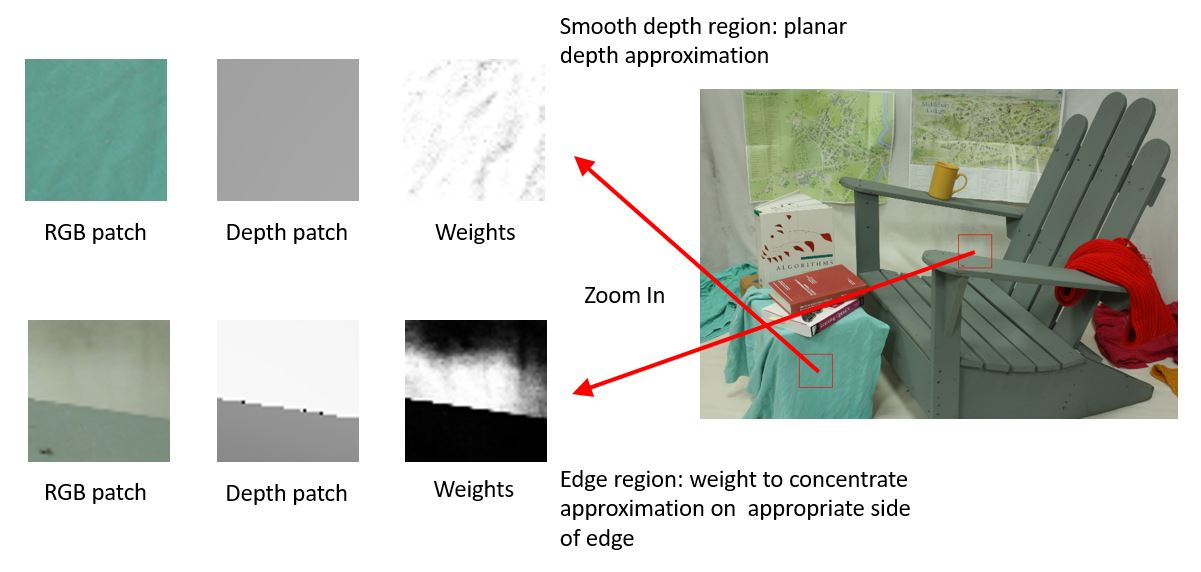
\includegraphics[width=0.95\linewidth]{depth_interp/misc/zoomin.JPG}
\label{fig2:zoomin}
\caption{The intuitive interpretation for the proposed algorithm. Two patch, respectively cropped from the handle area and the box ara, display different patterns in depth maps. The intuition of the proposed method aims to construct a linear interpolation based on only pixels with the same object which is supposed to be similar in both depth and color.}
\end{figure}
\begin{figure}[htb]
\centering
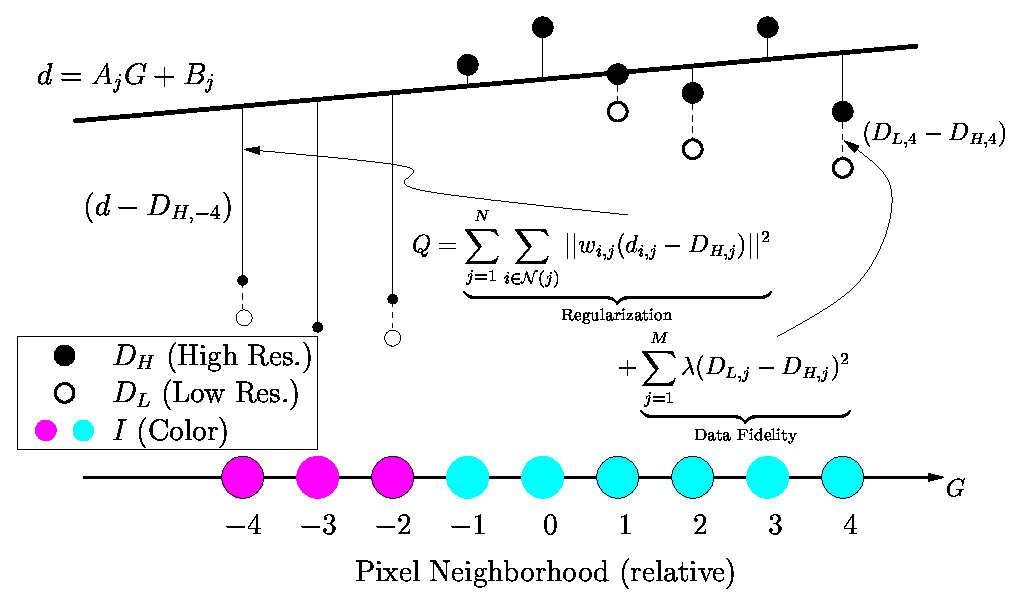
\includegraphics[width = 0.95\textwidth]{depth_interp/ProbFormulation.eps}
\vfill
\caption{The illustration of problem formulation in 1D. The magenta and cyan points show different color pixels in the patch of color image, and the circles around data points indicate the available low resolution depth values. The filled and un-filled circles mean the desired upsampled depth map and the input depth map, respectively, and the line is the fitting result on the example area. The weights are illustrated by the size of filled circles.}
\label{fig2:outline}
\end{figure}

To formally describe our algorithm we use the simplified 1D representation in Fig.~\ref{fig2:outline} that illustrates the contribution of one pixel to the objective function. The axis $G$ represents the relative pixel positions of points in local pixel neighborhood of the target pixel which is located at $G=0$. The low resolution depth map, denoted by $D_{L}$, is available at a subset of the pixel locations in the neighborhood as indicated in the figure and color values, denoted by $I$, form the high resolution RGB image. The goal is to estimate a high resolution depth map $D_H$. Our objective function is formulated as
\begin{equation}
Q = \sum_{j=1}^{N}{\sum_{i\in \mathcal{N}(j)}{||w_{i,j}(d_{i,j}-D_{H,i})||^2}}+\sum_{j=1}^{M}{{\lambda}(D_{L,j}-D_{H,j})^2},
\label{eq:2.1}
\end{equation}
where $j$ indexes the pixel locations in the upsampled image, $N$ is the number of pixels in the upsampled image, $M$ is the number of pixels in the low resolution depth map, $d_{i,j}$ is the value of linear fitting of pixel $i$ in the neighbor of pixel $j$, $D_{H,i}$ is the estimated depth at pixel $i$ in the neighbor of pixel $j$, and $D_{L,j}$ is the depth value at the pixel $j$ of the low resolution depth map, $w_{i,j}$ is the similarity metric of pixel $i$ and $j$, and $\lambda$ is the free parameter to control the relation of fidelity and smoothness. The local linear fit is defined as
\begin{equation}
d_{i,j} = A_{j}G_{i,j}+B_{j},
\label{eq:2.2}
\end{equation}
where $A_{j}$ and $B_{j}$ are the parameters for linear fitting at pixel $D_{H,j}$, $A_{j}$ is a 1-by-2 vector and $B_{j}$ is a scalar, and $G_{i,j}$ is a 2-by-1 vector denoting the relative coordinate of pixel $i$ in the neighbor window of pixel $j$. We define $G_{i,j}\overset{def}{=}\{(x,y)|-w_{s}<x<w_{s},-w_{s}<y<w_{s}\}$, where $w_{s}$ is the size of the window. The first term in~\eqref{eq:1} is the regularization term and the second term is the data fidelity. The formulation is readily extended to the hole filling problem by adding, to the fidelity penalty term, a product with the indicator function of non-missing points and pixel values.

The weights $w_{i,j}$ are defined as
\begin{equation}
w_{i,j} = \exp{-\frac{||I_{i}-I_{j}||^2}{2\sigma^2}},
\label{eq:2.4}
\end{equation}
where $I_{i}$ and $I_{j}$ are pixel values of the RGB image $I$ at corresponding position, and $\sigma$ controls the relative emphasis of pixel similarity in the allocation of weights. Alternative, formulations of the weights such as those used in non local mean or bilateral filter can also be used in the proposed framework. Unlike the typical bilateral filter, we do not use the distance decay term in~\eqref{eq:2.4} because the window we use is quite small comparing to the high resolution images. 

Our problem formulation and the algorithmic approach we use for the solution (described in the next section) are inspired by Levin's formulation of matting as an optimization problem~\cite{levin2008closed}, where the alpha channel is formulated as a weighted linear combination of neighboring color values. A key difference in our formulation is that the our weighted local linear fit is formulated in terms of the local relative {\em spatial} position for the neighborhood, whereas in~\cite{levin2008closed} the weighted linear fit is performed on the {\em color} values for the neighborhood pixels. 

\subsection{Optimization Solution}
\label{sec2.3.2}
%The optimization of this objective can be formulated as calculating the upsampling Laplacian matrix and solve the linear equation. 
Rewriting~\eqref{eq:2.1} in the matrix form, we obtain
\begin{equation}
Q = \sum_{j=1}^{N}{(W_{j}(D_{H,N_{j}}-GP_{j}^T))^2+{\lambda}F_{j}},
\label{eq:2.5}
\end{equation}
where $G = [G_j,1]$ and $P_{j} = [A_{j},B_{j}]^T$. $W_{j}$ is a diagonal matrix with $w_{i,j}$ being its diagonal entries. $D_{H,N_{j}}$ is the depth value in the patch\footnote{We pad the image to represent $G$ consistently at all positions.}. The matrix $P_{j}$ can be eliminated by replacing it in~\eqref{eq:2.5} by its optimal value 

\begin{equation}
\label{eq:2.6}
\begin{split}
P_{j} &=  {\argmin}_{P_{j}}{((W_{j}(D_{H,N_{j}}-GP_{j}^T))^2)}\\
&= (G^{T}W_{0,j}^{T}G)^{-1}G^{T}W_{0,j}^{T}D_{H,N_{j}},
\end{split}
\end{equation}
where $W_{0,j}$ is the diagonal matrix,
\begin{equation}
W_{0,j} = W_{j}^{T}W_{j},
\end{equation}
% \vspace*{-0.05in}
% \begin{equation*}
% W_{0,j} = W_{j}^{T}W_{j}.
% \vspace*{-0.05in}
% \end{equation*}

% As defined, $P_{j}$ is the fitting parameter based on the specific patch. By~\eqref{eq:6}, these terms have been expressed with known parameters.
Replacing $P_{j}$ in ~\eqref{eq:2.1} by~\eqref{eq:2.6}, we obtain,
\begin{equation}
Q = \sum_{j=1}^{N}{D_{H,N_{j}}^{T}(\overline{G_{j}}^{T}W_{0,j}\overline{G_{j}})D_{H,N_{j}}}+\sum_{j=1}^{M}{\lambda(D_{L,j}-D_{H,j})^2},
\label{eq:2.7}
\end{equation}
\begin{equation}
\overline{G_{j}}= E-G(G^{T}W_{0,j}^{T}G)^{-1}G^{T}W_{0,j},
\end{equation}
where $E$ denoting the identity matrix.
%can be expressed as
% \begin{equation*}
% \overline{G_{j}} = E-G(G^{T}W_{0,j}^{T}G)^{-1}G^{T}W_{0,j},
% \end{equation*}
% where $E$ is a identity matrix. At this point, all unknown parameters are eliminated and the optimization is just based on~\eqref{eq:5}.

%Because the objective function $Q$ is quadratic, 
The minimizer for the quadratic objective function $Q$ is readily obtained, specifically, as the solution to the linear equation,
\begin{equation}
LD+\lambda A(D-d) = 0,
\label{eq:2.8}
\end{equation}
where $L$ is the Laplacian matrix~\cite{merris1994laplacian},
\begin{equation}
L= \sum_{j=1}^{N}{\overline{G_{j}}^{T}W_{0,j}\overline{G_{j}}}
\label{eq:lpl}
\end{equation}
and $A$ is a diagonal matrix indicating the correspondence of pixels in low resolution map to the upsampled map. The derivation detail is listed in appendix~\ref{ap1}.
% is the 
% \begin{equation*}
% L = \sum_{j=1}^{N}{\overline{G_{j}}^{T}W_{0,j}\overline{G_{j}}},
% \end{equation*}
% and $A$ is a diagonal matrix indicating the correspondence of pixels in low resolution map to the upsampled map. $L$ is called the Laplacian matrix~\cite{merris1994laplacian}. With a proper window size, this linear equation is highly sparse and can be solved with conjugated gradient method.


%From the objective, we can see that depth map upsampling is similar to the matting problem~\cite{levin2008closed} with given strokes. The differences mainly lie in that in our algorithm, the depth value is linear to the relative position to the patch center and the color image working on the weight, while the matting algorithm directly formulates the alpha value on the linear combination of the color information.
\subsection{memory saving implementation}
\label{sec2.3.3}
In last section the optimization of the objective is formulated as an large sparse linear system, which can be efficiently solved with methods such as conjugate gradient solver. In practise, one important constraint for this method is that the Laplacian matrix and the successive processing, even though sparse, are very large and require a lot of memory. To reduce the memory requirement, we propose a computational efficiency improvement for the optimization, still exploiting the framework of conjugate gradient method~\cite{he2010fast,yu2014computational}.

Algorithm~\ref{algo:cg} describes the conjugate gradient algorithm for solving sparse linear systems. This algorithm is designed for solving symmetric and positive-definite linear systems, which is suitable for the optimization in our problem where the Laplacian matrix automatically satisfies the required condition. This method exploits the conjugate vectors with respect to $\textbf{A}$ and iteratively approximates the closest solution.

\begin{algorithm}
\SetKwData{Left}{left}
\SetKwData{This}{this}
\SetKwData{Up}{up}
\SetKwFunction{Union}{Union}
\SetKwFunction{FindCompress}{FindCompress}
\SetKwInOut{Input}{input}
\SetKwInOut{Output}{output}
\Input{Initial guess $\textbf{I}_0$, convergence threshold $\tau$}
\vspace{0.1in}
\Output{$\tilde{\textbf{I}}$ : estimate for $\textbf{I}$}
\vspace{0.1in}
\textbf{Procedure}\:
\vspace{0.1in}
\textbf{Initialize:} $\tilde{\textbf{I}}\leftarrow \textbf{I}_0$, $\textbf{r}_0\leftarrow \textbf{b}-\textbf{A}\tilde{\textbf{I}}$, $\textbf{p}_0\leftarrow \textbf{r}_0$, $j\leftarrow 0$\;
\vspace{0.1in}
\While{$\textbf{r}_j^T\textbf{r}_j > \tau |\textbf{I}|$}{\vspace{0.1in}$\alpha_j\leftarrow \frac{\textbf{r}_j^T\textbf{r}_j}{\textbf{p}_j^TA\textbf{p}_j}$\;\vspace{0.1in}
$\tilde{\textbf{I}}\leftarrow \tilde{\textbf{I}}+\alpha_j\textbf{p}_j$\;\vspace{0.1in}
$\textbf{r}_{j+1}\leftarrow \textbf{r}_j-\alpha_j \textbf{A}\textbf{p}_j$\;
\vspace{0.1in}
$\beta_j\leftarrow \frac{\textbf{r}_{j+1}^T\textbf{r}_{j+1}}{\textbf{r}_j^T\textbf{r}_j}$\;
\vspace{0.1in}
$\textbf{p}_{j+1}\leftarrow \textbf{r}_{j+1}+\beta_j \textbf{p}_j$\;\vspace{0.1in}}\vspace{0.1in}
\caption{Solve the sparse linear system $\textbf{AI} = \textbf{b}$ using conjugate-gradient algorithm.}
\label{algo:cg}
\end{algorithm}

One bottleneck for the proposed depth upsampling algorithm is that, for high resolution images, the Laplacian matrix is beyond typical computers' memory, for example a mega-pixel image will require constructing a matrix of tera-entries. This problem can be effective solved with some modifications on the naive conjugate gradient method, namely calculating $\textbf{A}\textbf{p}_j$ in algorithm~\ref{algo:cg} without explicit constructing $\textbf{A}$, in our case the Laplacian matrix.

From ~\eqref{eq:lpl} we can obtain the the entry $L_{i,j}$ at the $i$th row and the $j$ column of the Laplacian matrix, 
\begin{equation}
L_{i,j} = \sum_{k|i,j\in N_{k}}{(\delta_{ij}w_{ki}-w_{ki}w_{kj}(G_{i}-k_{0})C_{k}(G_{j}-k_{0}))},
\label{eq:2.cgs_partial1}
\end{equation}
where $N_{k}$ is the neighbour of pixel $k$, whose range is specified by the window size, $w_{ki}$ is the weigh of pixel $k$ to pixel $i$ and $j$, $\delta_{ij}$ is the Kronecker delta , $C_{k}$ is the inverse of $\overline{G_{j}}^{T}W_{0,j}\overline{G_{j}}$ of pixel $k$, $G_{i}$ is relative coordinate of pixel $i$ to $k$, and $k_0$ is the the global coordinate of the pixel $k$. Then we break the summation stepwise, first computing, 
\begin{equation}
a_{k} = C_{k}(\sum_{j\in N_{k}}{w_{kj}}G_{j}P_{j}-k\overline{p_{k}}),
\label{eq:2.cgs_partial2}
\end{equation}
where $P_j$ is the $i$th entry of vector $P$, and $\overline{p_{k}}$ is the average of $P_j$ in $N_{k}$. then,
\begin{equation}
b_{k} = k_{0}a_{k},
\label{eq:2.cgs_partial3}
\end{equation}
at the last step, combine $a_k$ and $b_k$ to obtain $(Lp)_{i}$, the entry at the $i$th column of vector $Lp$,
\begin{equation}
(Lp)_{i} = \sum{\delta_{ij}w_{ki}P_{i}}-G_{i}\sum_{k\in N_{i}}{a_{k}w_{ki}}+\sum_{k\in N_{i}}{b_{k}w_{ki}},
\label{eq:2.cgs_final}
\end{equation}
further, the inverse $C_k$ can be expressed as,
\begin{landscape}
\begin{equation}
C = \left \{
  \begin{tabular}{ccc}
  $\textbf{y}^T\textbf{wy1}^T\textbf{w1}-\textbf{y}^T\textbf{w11}^T\textbf{wy}$ & $\textbf{y}^T\textbf{w11}^T\textbf{wx}-\textbf{y}^T\textbf{wx1}^T\textbf{w1}$ & $\textbf{y}^T\textbf{wx1}^T\textbf{wy}-\textbf{y}^T\textbf{wy1}^T\textbf{wx}$ \\
  $\textbf{x}^T\textbf{w11}^T\textbf{wy}-\textbf{x}^T\textbf{wy1}^T\textbf{w1}$ & $\textbf{x}^T\textbf{wx1}^T\textbf{w1}-\textbf{x}^T\textbf{w11}^T\textbf{wx}$ & $\textbf{x}^T\textbf{wy1}^T\textbf{wx}-\textbf{x}^T\textbf{wx1}^T\textbf{wy}$ \\
  $\textbf{x}^T\textbf{wyy}^T\textbf{w1}-\textbf{x}^T\textbf{w1y}^T\textbf{wy}$ & $\textbf{x}^T\textbf{w1y}^T\textbf{wx}-\textbf{x}^T\textbf{wxy}^T\textbf{w1}$ & $\textbf{x}^T\textbf{wxy}^T\textbf{wy}-\textbf{x}^T\textbf{wyy}^T\textbf{wx}$
  \end{tabular}
\right \},\\
\label{eq:2.inverse}
\end{equation}
or more compactly as the minor of the matrix:\\
\begin{equation}
C = \left \{
  \begin{tabular}{ccc}
  $M_{1,1}$ & $M_{1,2}$ & $M_{1,3}$ \\
  $M_{2,1}$ & $M_{2,2}$ & $M_{2,3}$ \\
  $M_{3,1}$ & $M_{3,2}$ & $M_{3,3}$
  \end{tabular}
\right \},
\end{equation}
here the normalization term omitted.
\end{landscape}
Substitute the update step of $p_{j+1}$ in algorithm~\ref{algo:cg} with~\eqref{eq:2.cgs_final} we can get the version for optimization the proposed depth upsampling algorithm. The derivation detail is listed in appendix~\ref{ap2}.

In colorization problem the summation in~\eqref{eq:2.cgs_partial2},~\eqref{eq:2.cgs_partial3}, and ~\eqref{eq:2.cgs_final} can be efficiently calculated by integral image techniques and dynamic programming. This step is possible as that the formulation in colorization utilizes a fixed summation table; but in our case, the $G_{j}w_{kj}$ is a summed table of localized filters $w_{k}$, which means that the values re-used in summed table is no longer applicable here. This restriction limits the acceleration of computing but still allows the memory saving. By this implementation the required memory for a two mega-pixel image is reduced from 60GB to 2GB memory. With parallel computation, this method can have a good balance in memory usage and time consumption.


\section{experimental results}
\label{sec:2.result}
We test our algorithm on the Middlebury (stereo) dataset~\cite{scharstein2003high,scharstein2007learning,hirschmuller2007evaluation,scharstein2014high}, which provides high resolution RGB images of multiple views and corresponding disparity maps, which are used as the ground truth in our experiment. We use a window size of $7\times 7$ ($\equiv N=49$), and $\lambda=10^5$. The RGB-D images are zero-padded for consistent use of~\eqref{eq:5}, and the padded area is cropped out in the final results. The parameter $\sigma^2$ in~\eqref{eq:4} for computation of the weights $w_{i,j}$ is set to one third of the local variance in each window. In each patch, the weight of the center pixel is set to $10^{-5}$. We use the built-in Matlab conjugate gradient solver (\emph{cgs}) for solving~\eqref{eq:8} (a tolerance of $10^{-10}$ and maximum number of iteration $10^4$ were used).
\subsection{Qualitative and Quantitative Results}
The proposed algorithm is both suitable for hole filling for single disparity map and depth map upsampling, as indicated earlier. In this part, we first visually examine the performance of filling holes in depth map, as shown in Fig.~\ref{fig:quali_rst}. From the images in the last column, we can find that the holes, which correspond to the occluded area in the disparity map, are well filled. Unlike traditional interpolation methods, our algorithm is able to fix the holes in the depth images, so as to keep the consistency of depth map edges with those in the RGB images and avoid smoothing in such areas. For example, see the third row of Fig.~\ref{fig:quali_rst}. The missing points along the wall are well fitted to the two sides, and not blurred as a large patch.
% Behind we show results of the interpolation.
\begin{figure}[htb]
% \begin{minipage}[b]{0.3\linewidth}
%   \centering
%   \centerline{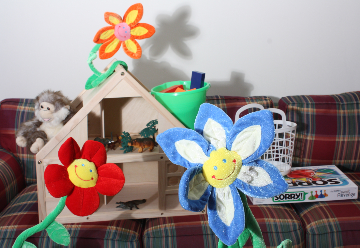
\includegraphics[width=2.7cm]{quali_rst/img_Flowers-perfect.png}}
% %  \vspace{1.5cm}
% %   \centerline{(a)}\medskip
% \end{minipage}
% %
% \hfill
% \begin{minipage}[b]{0.3\linewidth}
%   \centering
%   \centerline{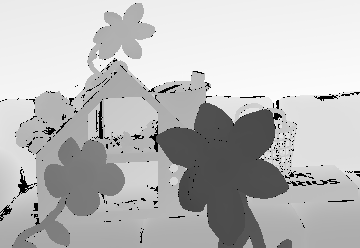
\includegraphics[width=2.7cm]{quali_rst/n_hf_Flowers-perfect.png}}
% %  \vspace{1.5cm}
% %   \centerline{(b)}\medskip
% \end{minipage}
% \hfill
% \begin{minipage}[b]{0.3\linewidth}
%   \centering
%   \centerline{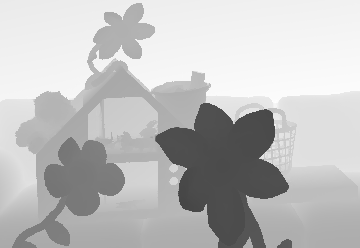
\includegraphics[width=2.7cm]{quali_rst/hf_Flowers-perfect.png}}
% %  \vspace{1.5cm}
% %   \centerline{(c)}\medskip
% \end{minipage}
% \vfill
\begin{minipage}[b]{0.3\linewidth}
  \centering
  \centerline{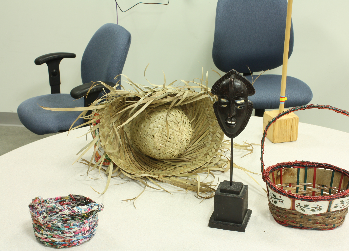
\includegraphics[width=4.2cm]{depth_interp/quali_rst/img_Mask-perfect.png}}
%  \vspace{1.5cm}
%   \centerline{(a)}\medskip
\end{minipage}
%
\hfill
\begin{minipage}[b]{0.3\linewidth}
  \centering
  \centerline{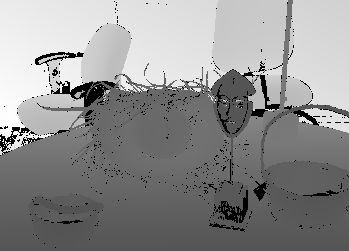
\includegraphics[width=4.2cm]{depth_interp/quali_rst/n_hf_Mask-perfect.png}}
%  \vspace{1.5cm}
%   \centerline{(b)}\medskip
\end{minipage}
\hfill
\begin{minipage}[b]{0.3\linewidth}
  \centering
  \centerline{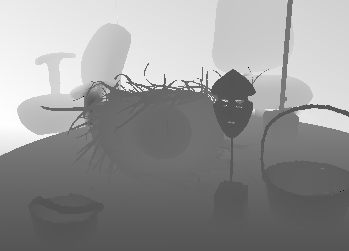
\includegraphics[width=4.2cm]{depth_interp/quali_rst/hf_Mask-perfect.png}}
%  \vspace{1.5cm}
%   \centerline{(c)}\medskip
\end{minipage}
\vfill
% \begin{minipage}[b]{0.3\linewidth}
%   \centering
%   \centerline{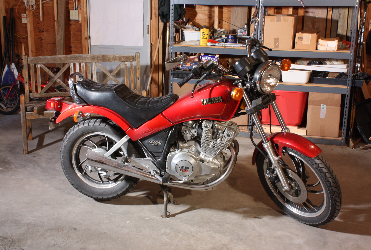
\includegraphics[width=2.7cm]{quali_rst/img_Motorcycle-perfect.png}}
% %  \vspace{1.5cm}
% %   \centerline{(a)}\medskip
% \end{minipage}
% %
% \hfill
% \begin{minipage}[b]{0.3\linewidth}
%   \centering
%   \centerline{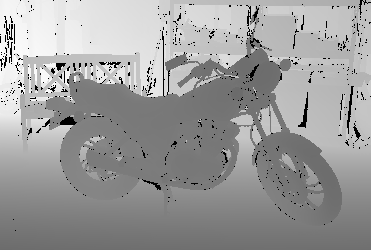
\includegraphics[width=2.7cm]{quali_rst/n_hf_Motorcycle-perfect.png}}
% %  \vspace{1.5cm}
% %   \centerline{(b)}\medskip
% \end{minipage}
% \hfill
% \begin{minipage}[b]{0.3\linewidth}
%   \centering
%   \centerline{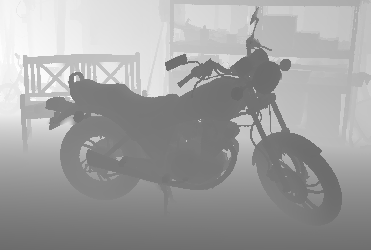
\includegraphics[width=2.7cm]{quali_rst/hf_Motorcycle-perfect.png}}
% %  \vspace{1.5cm}
% %   \centerline{(c)}\medskip
% \end{minipage}
% \vfill
\begin{minipage}[b]{0.3\linewidth}
  \centering
  \centerline{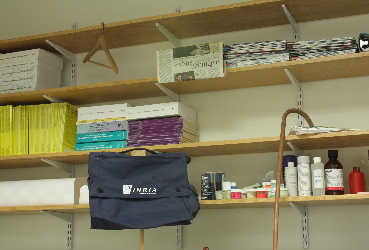
\includegraphics[width=4.2cm]{depth_interp/quali_rst/img_Shelves-perfect.png}}
%  \vspace{1.5cm}
%   \centerline{(a)}\medskip
\end{minipage}
%
\hfill
\begin{minipage}[b]{0.3\linewidth}
  \centering
  \centerline{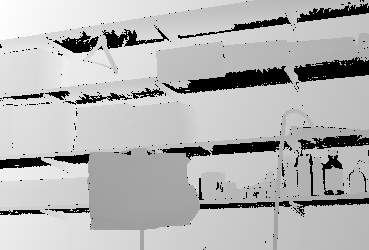
\includegraphics[width=4.2cm]{depth_interp/quali_rst/n_hf_Shelves-perfect.png}}
%  \vspace{1.5cm}
%   \centerline{(b)}\medskip
\end{minipage}
\hfill
\begin{minipage}[b]{0.3\linewidth}
  \centering
  \centerline{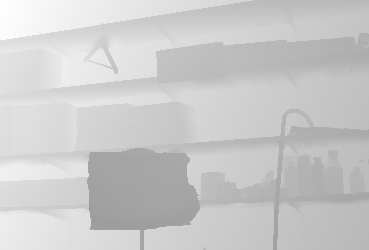
\includegraphics[width=4.2cm]{depth_interp/quali_rst/hf_Shelves-perfect.png}}
%  \vspace{1.5cm}
%   \centerline{(c)}\medskip
\end{minipage}
\vfill
\begin{minipage}[b]{0.3\linewidth}
  \centering
  \centerline{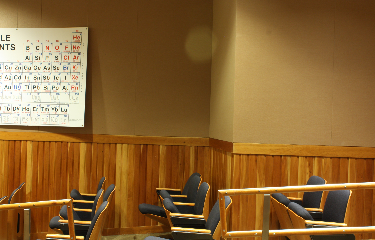
\includegraphics[width=4.2cm]{depth_interp/quali_rst/img_Classroom1-perfect.png}}
%  \vspace{1.5cm}
%   \centerline{(a)}\medskip
\end{minipage}
%
\hfill
\begin{minipage}[b]{0.3\linewidth}
  \centering
  \centerline{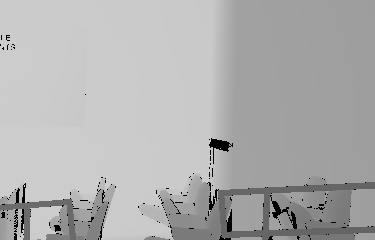
\includegraphics[width=4.2cm]{depth_interp/quali_rst/n_hf_Classroom1-perfect.png}}
%  \vspace{1.5cm}
%   \centerline{(b)}\medskip
\end{minipage}
\hfill
\begin{minipage}[b]{0.3\linewidth}
  \centering
  \centerline{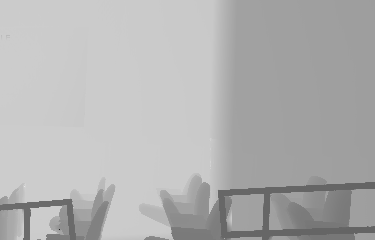
\includegraphics[width=4.2cm]{depth_interp/quali_rst/hf_Classroom1-perfect.png}}
%  \vspace{1.5cm}
%   \centerline{(c)}\medskip
\end{minipage}
\vfill
\begin{minipage}[b]{0.3\linewidth}
  \centering
  \centerline{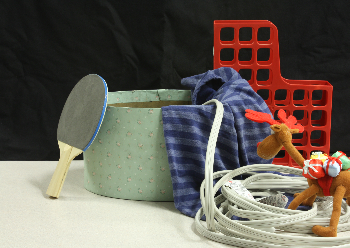
\includegraphics[width=4.2cm]{depth_interp/quali_rst/img_Cable-perfect.png}}
%  \vspace{1.5cm}
%   \centerline{(a)}\medskip
\end{minipage}
%
\hfill
\begin{minipage}[b]{0.3\linewidth}
  \centering
  \centerline{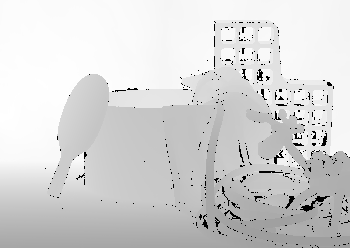
\includegraphics[width=4.2cm]{depth_interp/quali_rst/n_hf_Cable-perfect.png}}
%  \vspace{1.5cm}
%   \centerline{(b)}\medskip
\end{minipage}
\hfill
\begin{minipage}[b]{0.3\linewidth}
  \centering
  \centerline{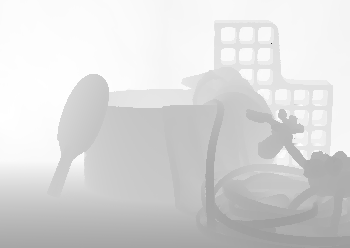
\includegraphics[width=4.2cm]{depth_interp/quali_rst/hf_Cable-perfect.png}}
%  \vspace{1.5cm}
%   \centerline{(c)}\medskip
\end{minipage}
\vspace*{-0.10in}
\caption{Qualitative results of the hole filling ability of our algorithm, tested on Middlebury stereo dataset 2014~\cite{scharstein2014high}. The first column shows the input high resolution color images and the second column shows the corresponding depth maps. The results are shown in the last column. The images are processed at a low resolution of approximate 60k to 80k pixels.}
\label{fig:quali_rst}
\end{figure}
\begin{figure*}[t]
\begin{minipage}[b]{1.0\linewidth}
  \centering
  \centerline{\includegraphics[width=6cm]{depth_interp/quan_hf/Art.png}}
%  \vspace{1.5cm}
%   \centerline{(a)}\medskip
\end{minipage}
%
\vfill
\begin{minipage}[b]{0.48\linewidth}
  \centering
  \centerline{\includegraphics[width=5.5cm]{depth_interp/quan_nhf/gt.png}}
%  \vspace{1.5cm}
%   \centerline{(a)}\medskip
\end{minipage}
\hfill
\begin{minipage}[b]{0.48\linewidth}
  \centering
  \centerline{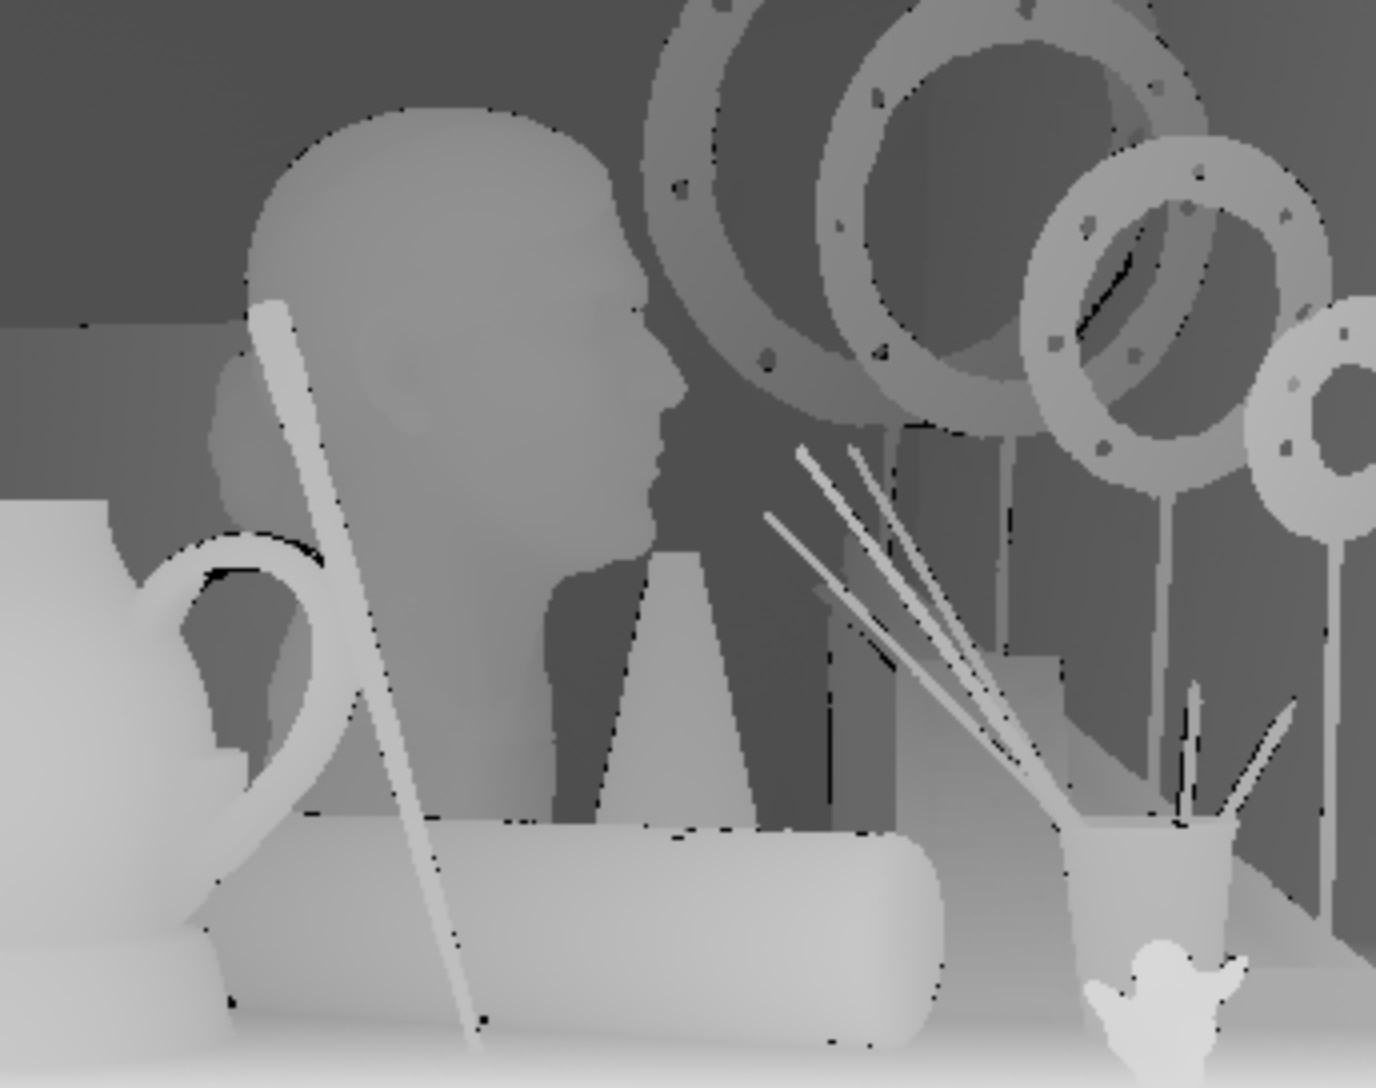
\includegraphics[width=5.5cm]{depth_interp/quan_nhf/bl.png}}
%  \vspace{1.5cm}
%   \centerline{(a)}\medskip
\end{minipage}
%
\vfill
\begin{minipage}[b]{0.48\linewidth}
  \centering
  \centerline{\includegraphics[width=5.5cm]{depth_interp/quan_nhf/bc.png}}
%  \vspace{1.5cm}
%   \centerline{(b)}\medskip
\end{minipage}
\hfill
\begin{minipage}[b]{0.48\linewidth}
  \centering
  \centerline{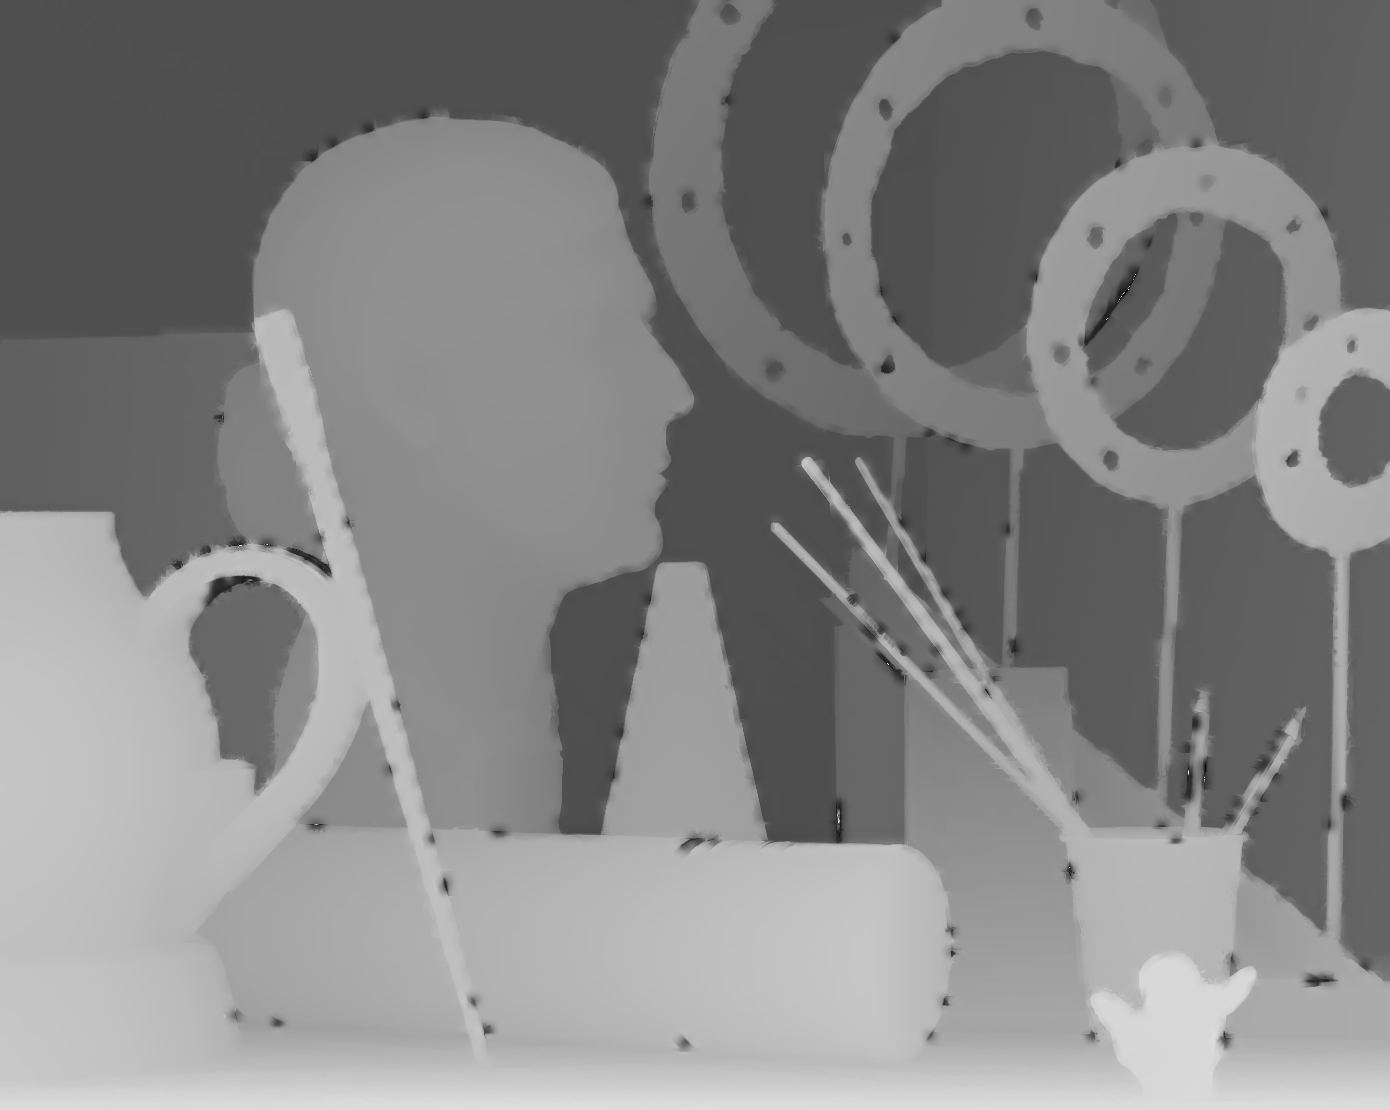
\includegraphics[width=5.5cm]{depth_interp/quan_nhf/yang.png}}
%  \vspace{1.5cm}
%   \centerline{(a)}\medskip
\end{minipage}
%
\vfill
\begin{minipage}[b]{0.48\linewidth}
  \centering
  \centerline{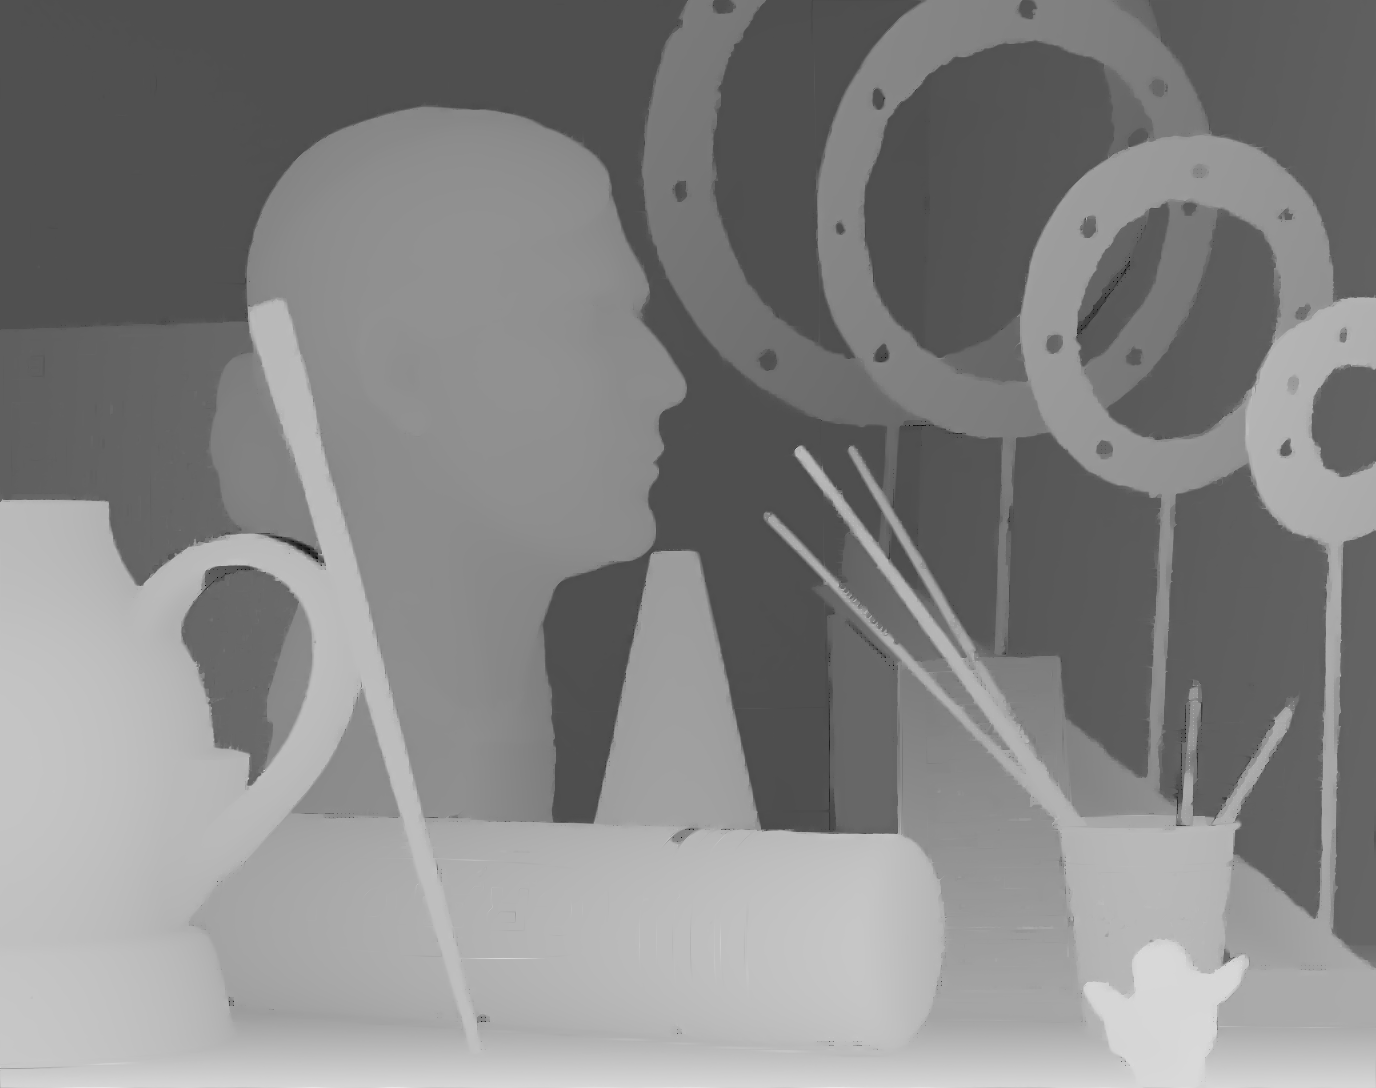
\includegraphics[width=5.5cm]{depth_interp/quan_nhf/tgv.png}}
%  \vspace{1.5cm}
%   \centerline{(a)}\medskip
\end{minipage}
%
\hfill
\begin{minipage}[b]{0.48\linewidth}
  \centering
  \centerline{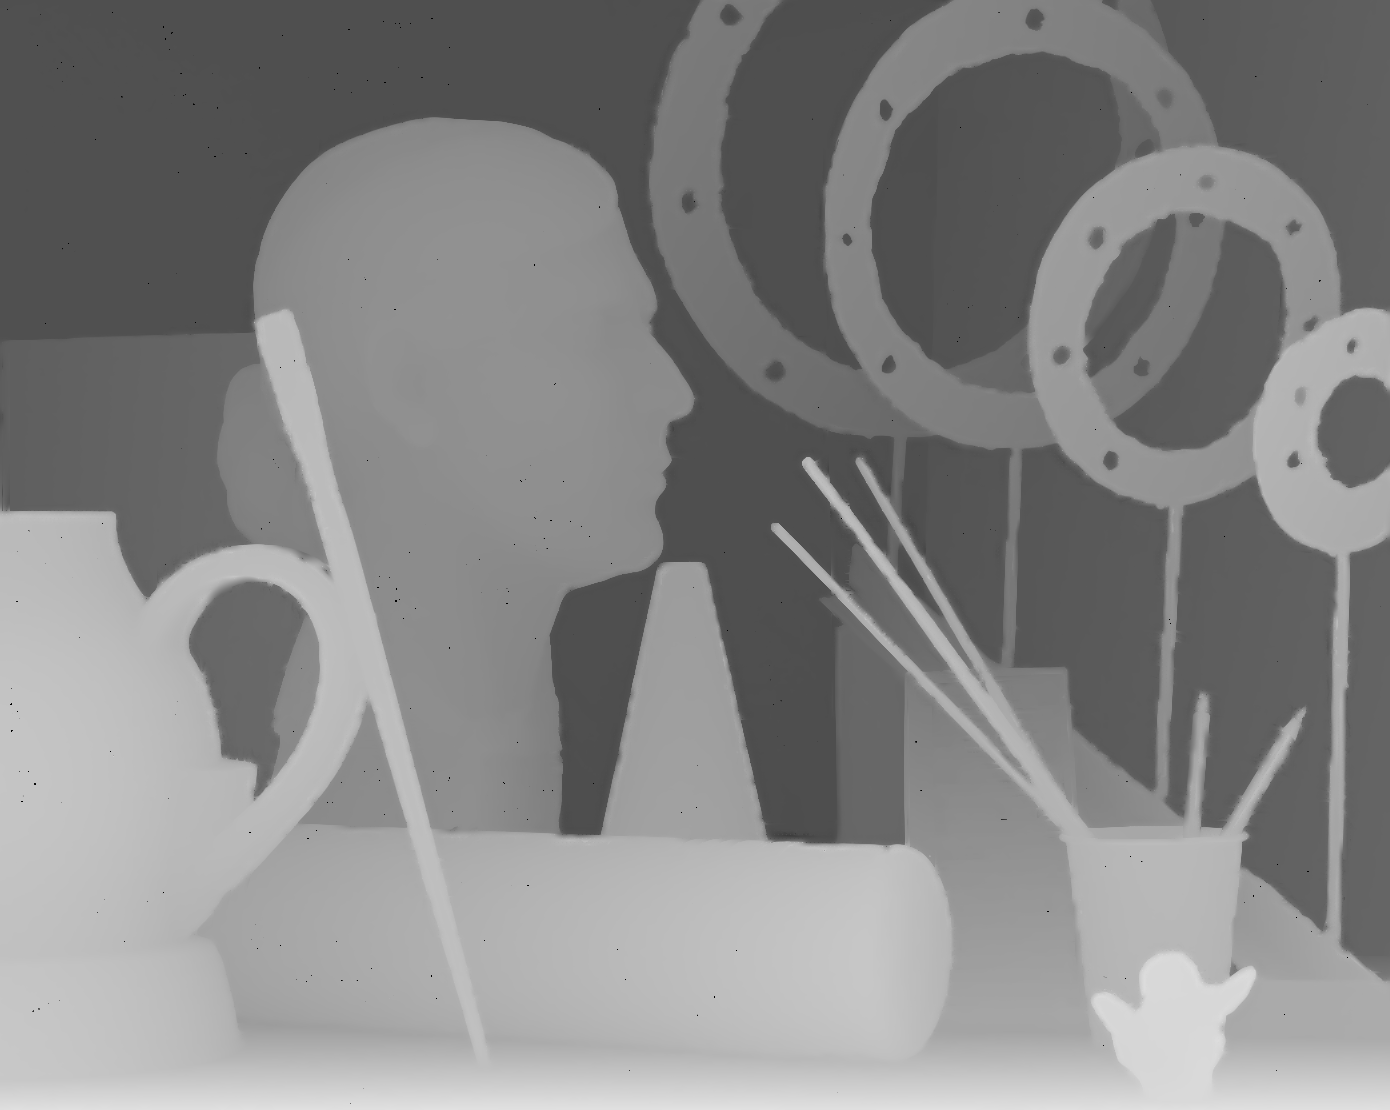
\includegraphics[width=5.5cm]{depth_interp/quan_nhf/our.png}}
%  \vspace{1.5cm}
%   \centerline{(b)}\medskip
\end{minipage}
\vfill
\label{fig2:art}
\caption{Visual comparison of different algorithm tested on Middlebury dataset~\cite{scharstein2003high} at $4\times$ upsampling rate. Column from left to right: RGB images, ground truth, and the results of: bilinear, bicubic, IBL~\cite{yang2014color}, TGV~\cite{ferstl2013image} and proposed; row from top to bottom: Art, Books, and Moebius.}
\end{figure*}
\begin{figure*}[t]
\begin{minipage}[b]{1\linewidth}
  \centering
  \centerline{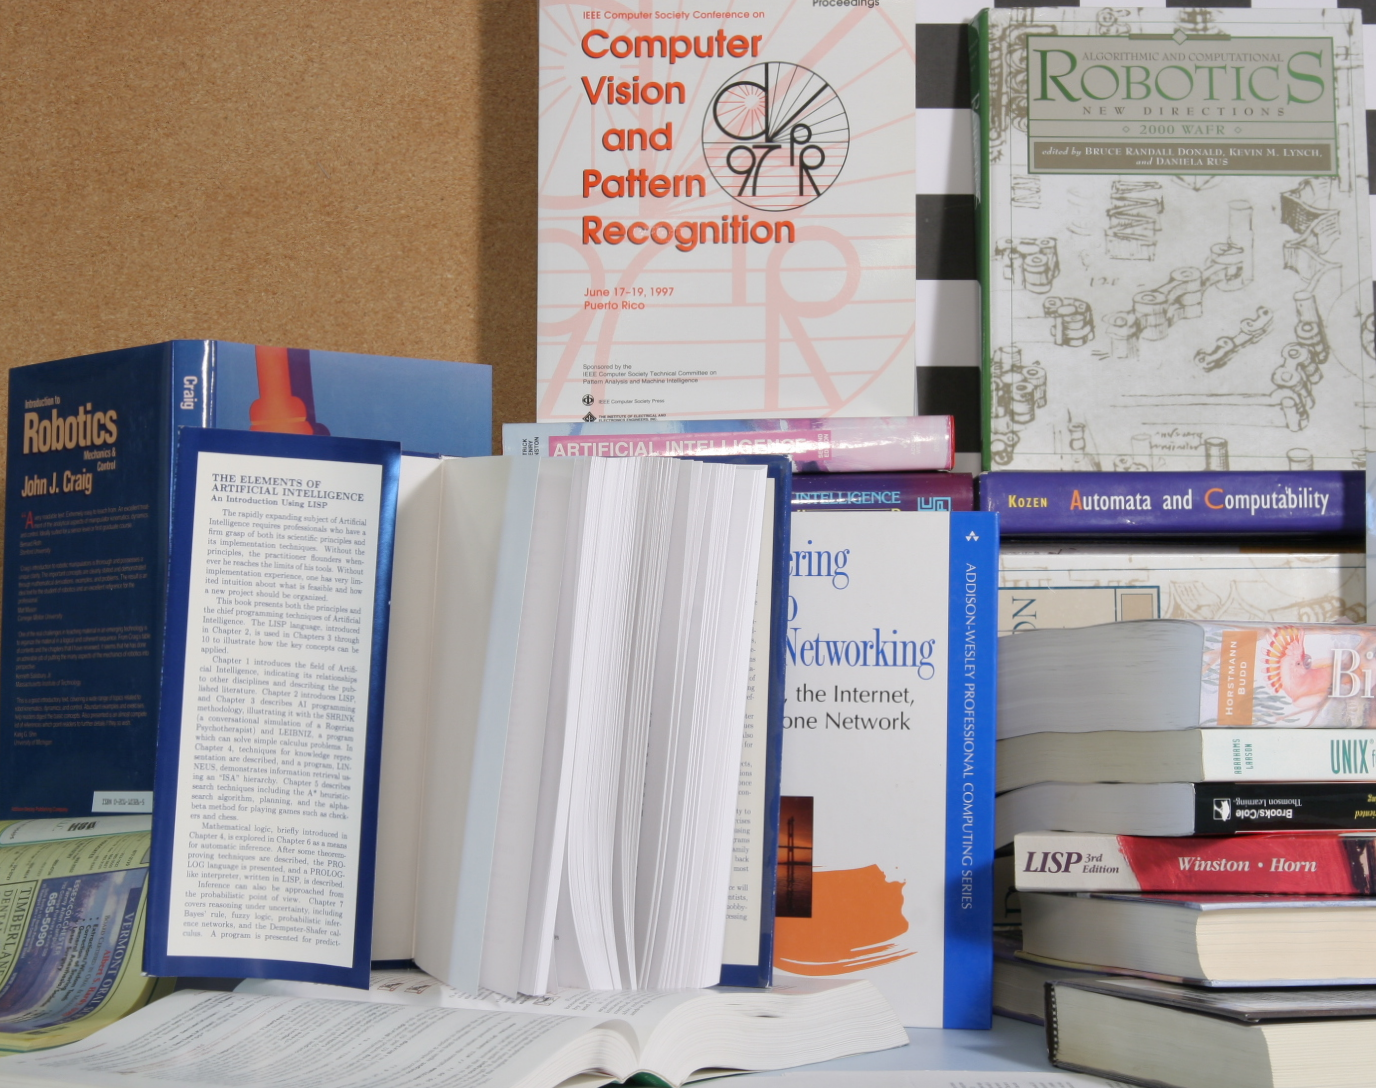
\includegraphics[width=6cm]{depth_interp/quan_nhf_books/Books.png}}
%  \vspace{1.5cm}
%   \centerline{(c)}\medskip
\end{minipage}
\hfill
\begin{minipage}[b]{0.48\linewidth}
  \centering
  \centerline{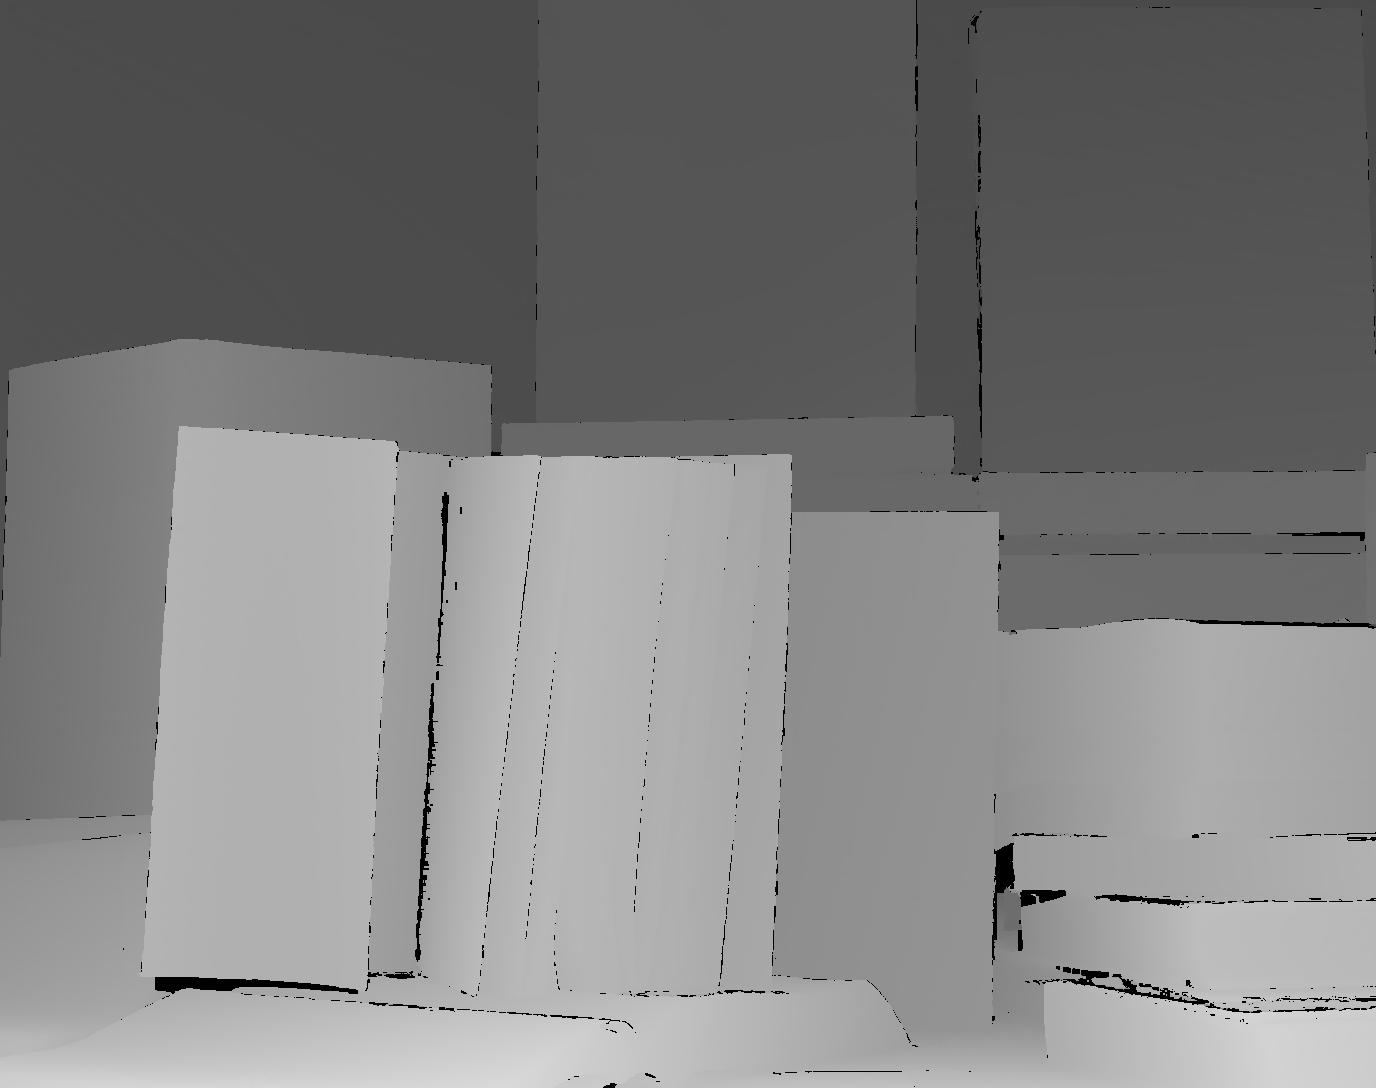
\includegraphics[width=5.5cm]{depth_interp/quan_nhf_books/gt.png}}
%  \vspace{1.5cm}
%   \centerline{(c)}\medskip
\end{minipage}
\hfill
\begin{minipage}[b]{0.48\linewidth}
  \centering
  \centerline{\includegraphics[width=5.5cm]{depth_interp/quan_nhf_books/bl.png}}
%  \vspace{1.5cm}
%   \centerline{(a)}\medskip
\end{minipage}
%
\hfill
\begin{minipage}[b]{0.48\linewidth}
  \centering
  \centerline{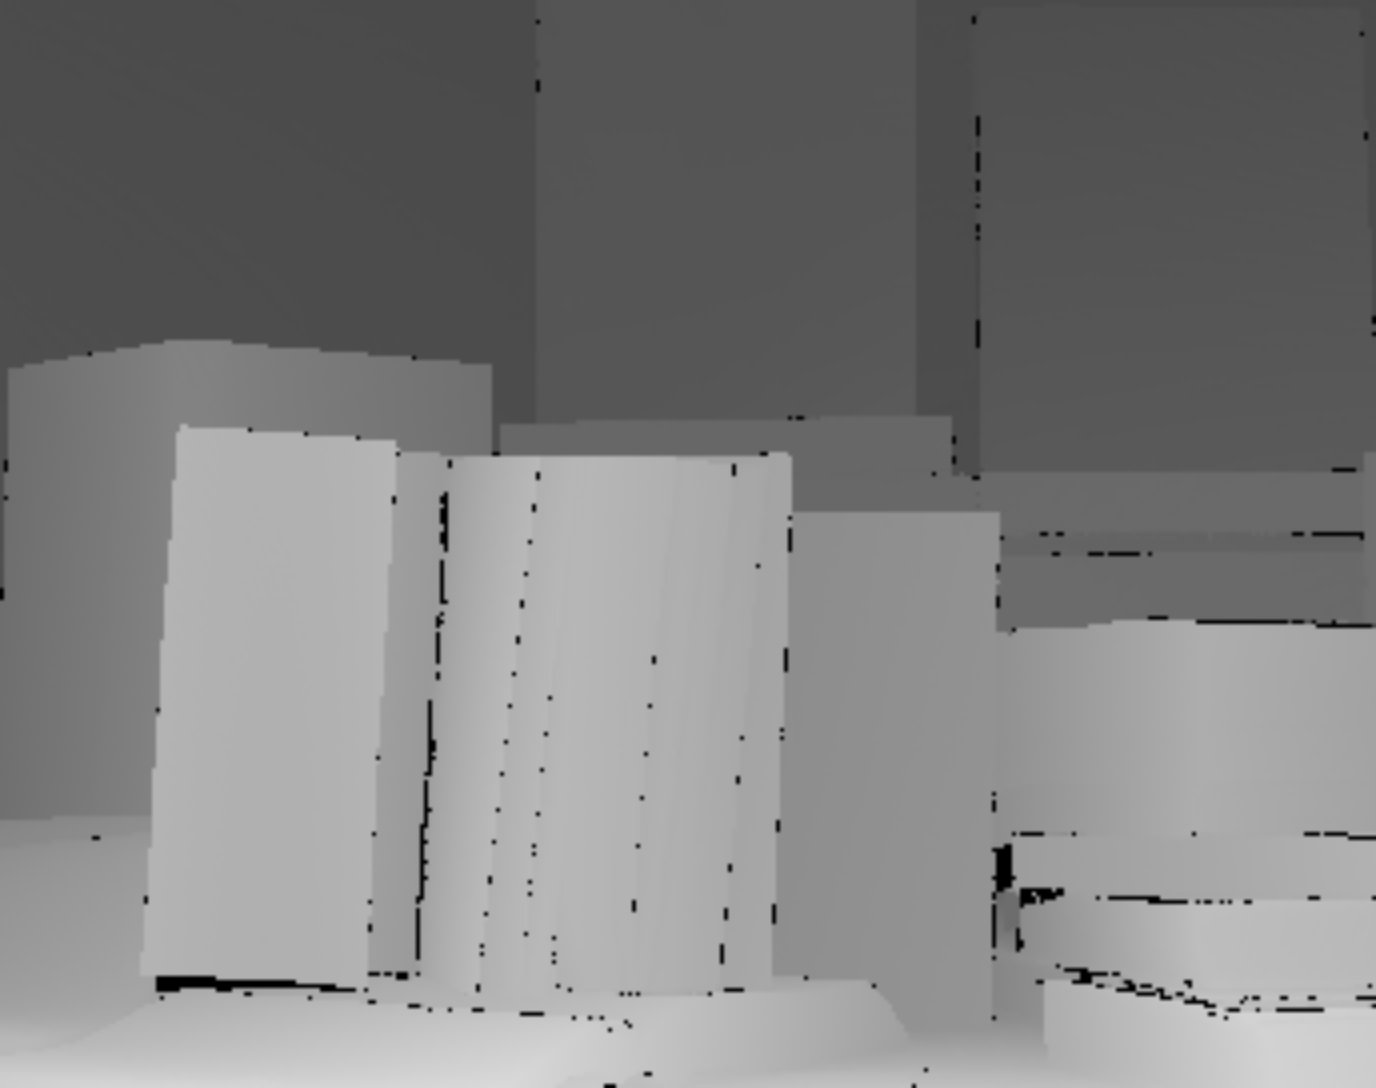
\includegraphics[width=5.5cm]{depth_interp/quan_nhf_books/bc.png}}
%  \vspace{1.5cm}
%   \centerline{(b)}\medskip
\end{minipage}
\hfill
\begin{minipage}[b]{0.48\linewidth}
  \centering
  \centerline{\includegraphics[width=5.5cm]{depth_interp/quan_nhf_books/yang.png}}
%  \vspace{1.5cm}
%   \centerline{(a)}\medskip
\end{minipage}
%
\hfill
\begin{minipage}[b]{0.48\linewidth}
  \centering
  \centerline{\includegraphics[width=5.5cm]{depth_interp/quan_nhf_books/tgv.png}}
%  \vspace{1.5cm}
%   \centerline{(a)}\medskip
\end{minipage}
%
\hfill
\begin{minipage}[b]{0.48\linewidth}
  \centering
  \centerline{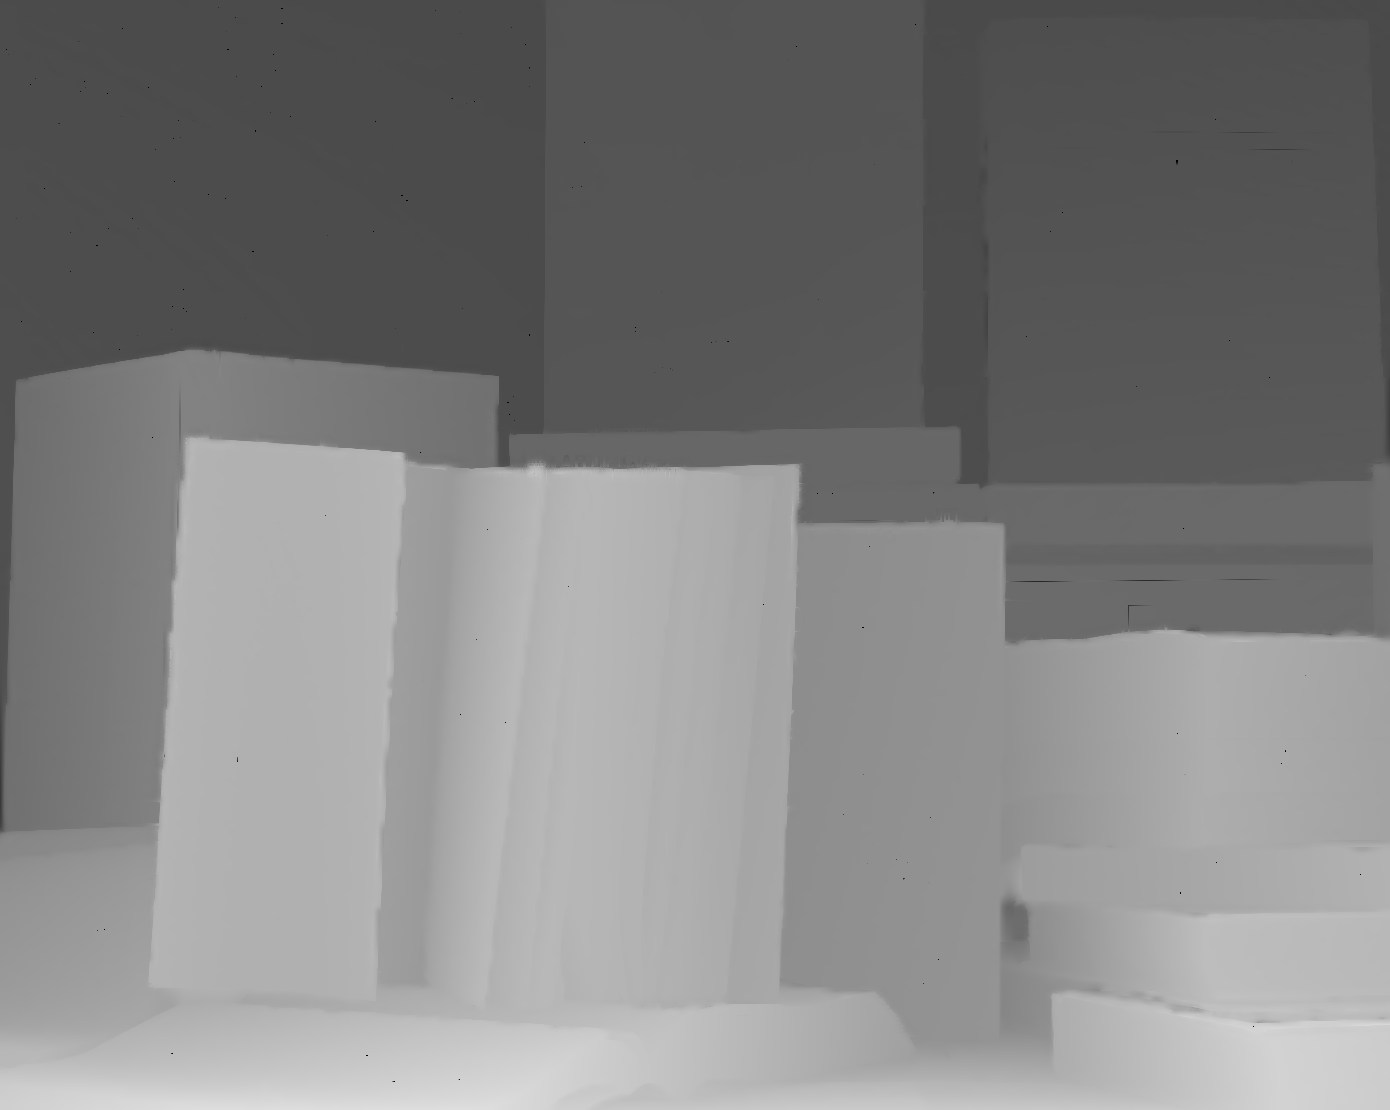
\includegraphics[width=5.5cm]{depth_interp/quan_nhf_books/our.png}}
%  \vspace{1.5cm}
%   \centerline{(b)}\medskip
\end{minipage}
\vfill
\label{fig2:books}
\caption{Visual comparison of different algorithm tested on Middlebury dataset~\cite{scharstein2003high} at $4\times$ upsampling rate. Column from left to right: RGB images, ground truth, and the results of: bilinear, bicubic, IBL~\cite{yang2014color}, TGV~\cite{ferstl2013image} and proposed; row from top to bottom: Art, Books, and Moebius.}
\end{figure*}
\begin{figure*}[t]
\begin{minipage}[b]{1\linewidth}
  \centering
  \centerline{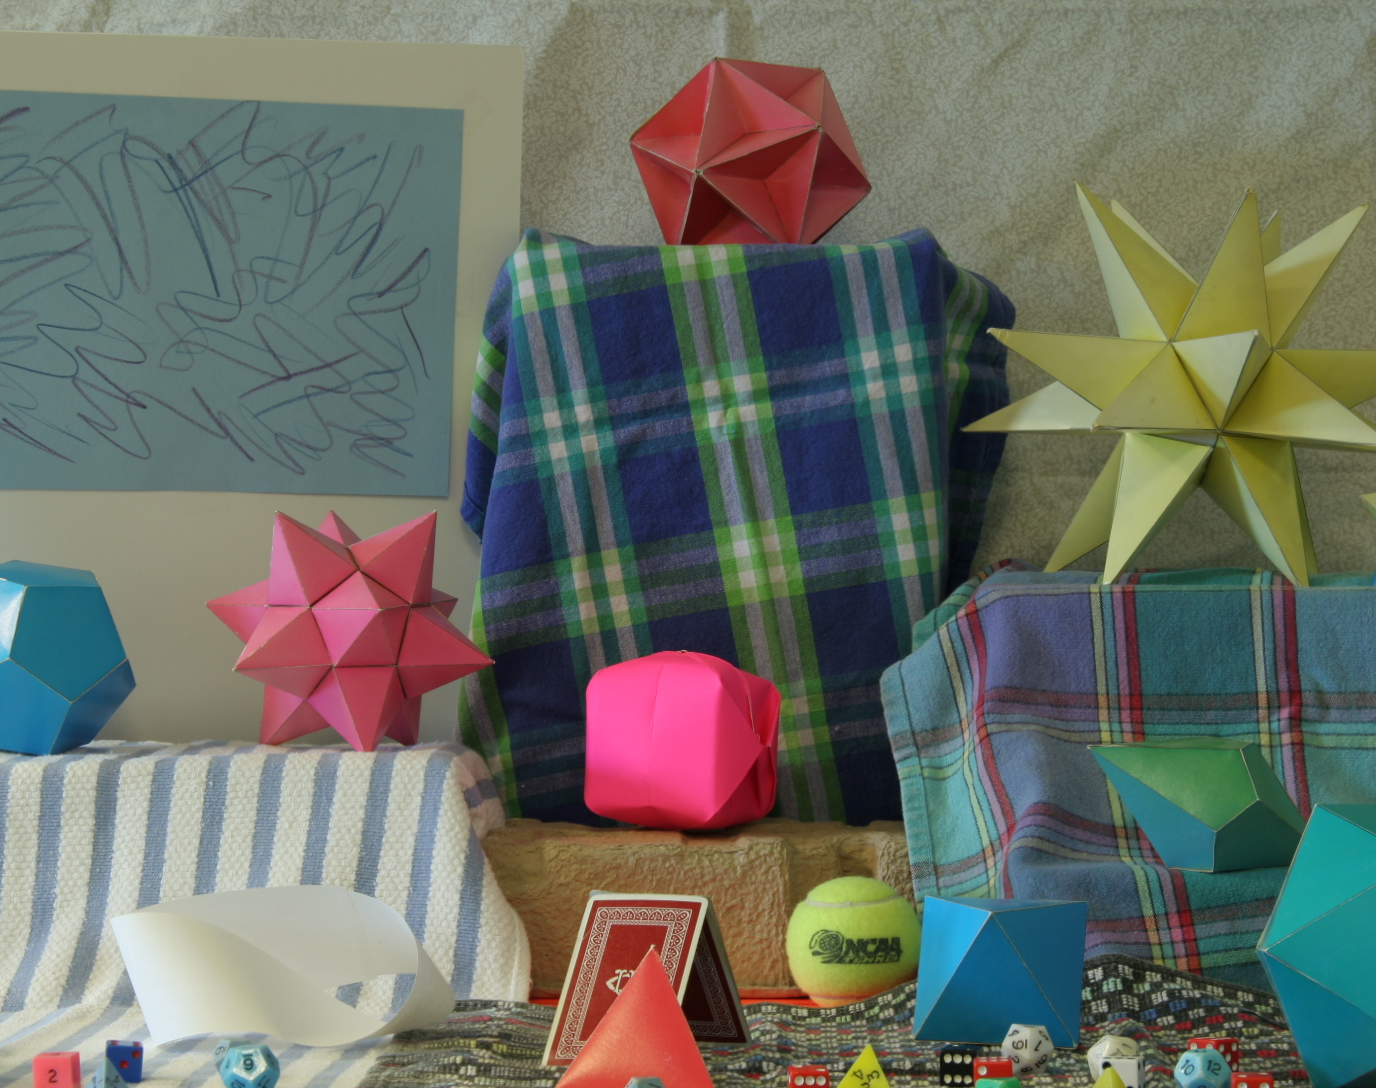
\includegraphics[width=6cm]{depth_interp/quan_nhf_moebius/Moebius.png}}
%  \vspace{1.5cm}
%   \centerline{(c)}\medskip
\end{minipage}
\hfill
\begin{minipage}[b]{0.48\linewidth}
  \centering
  \centerline{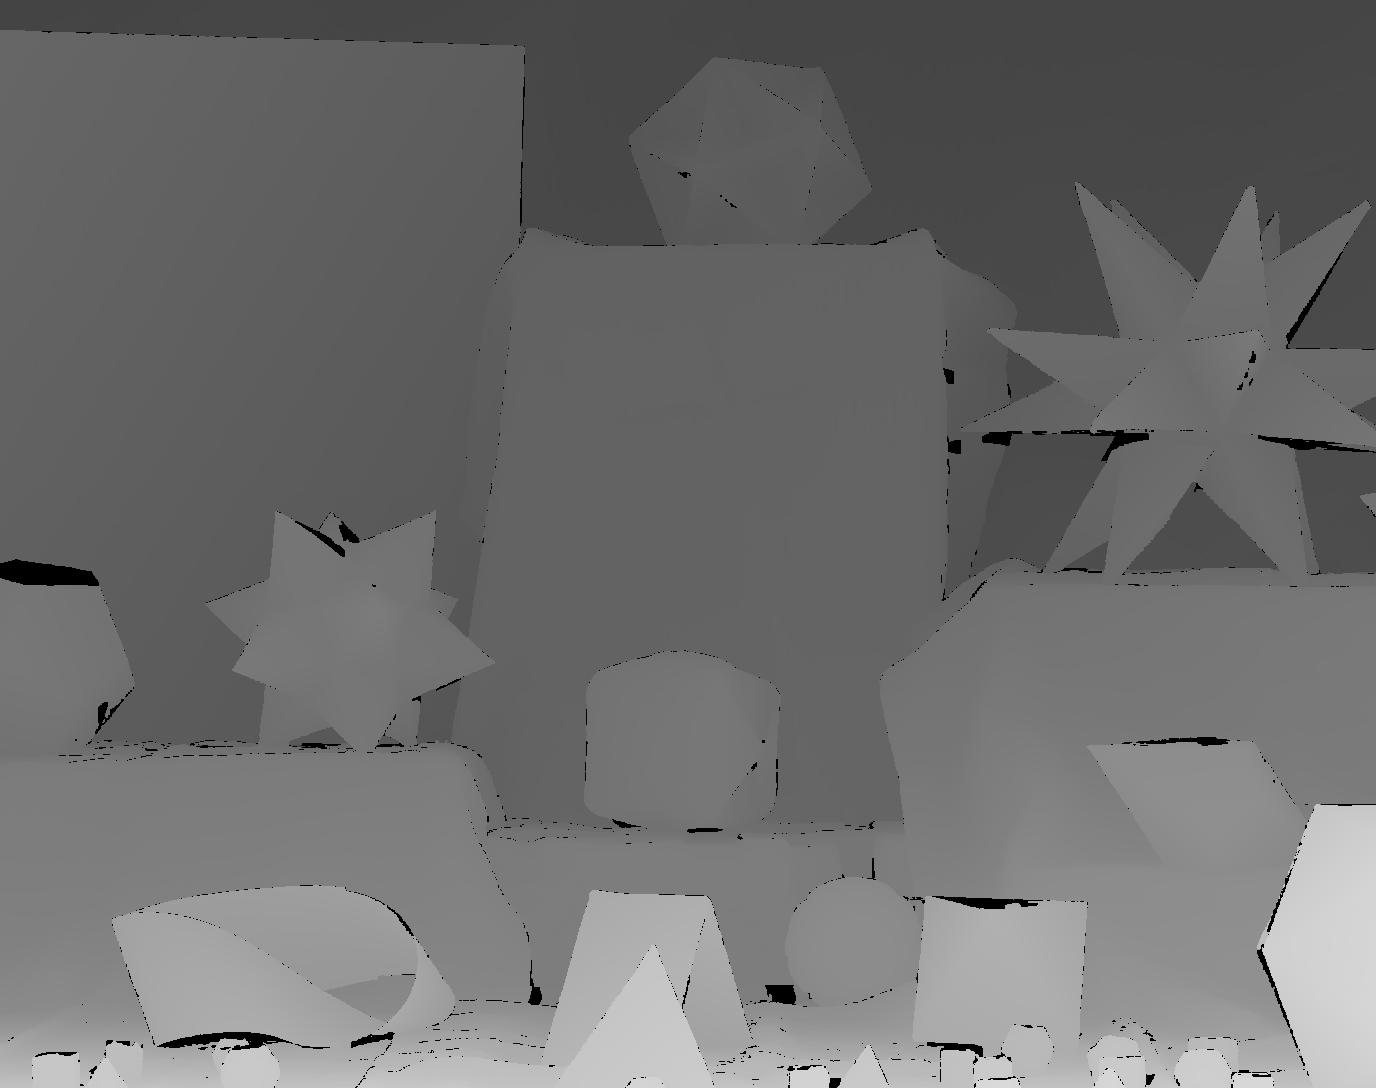
\includegraphics[width=5.5cm]{depth_interp/quan_nhf_moebius/gt.png}}
%  \vspace{1.5cm}
%   \centerline{(c)}\medskip
\end{minipage}
\hfill
\begin{minipage}[b]{0.48\linewidth}
  \centering
  \centerline{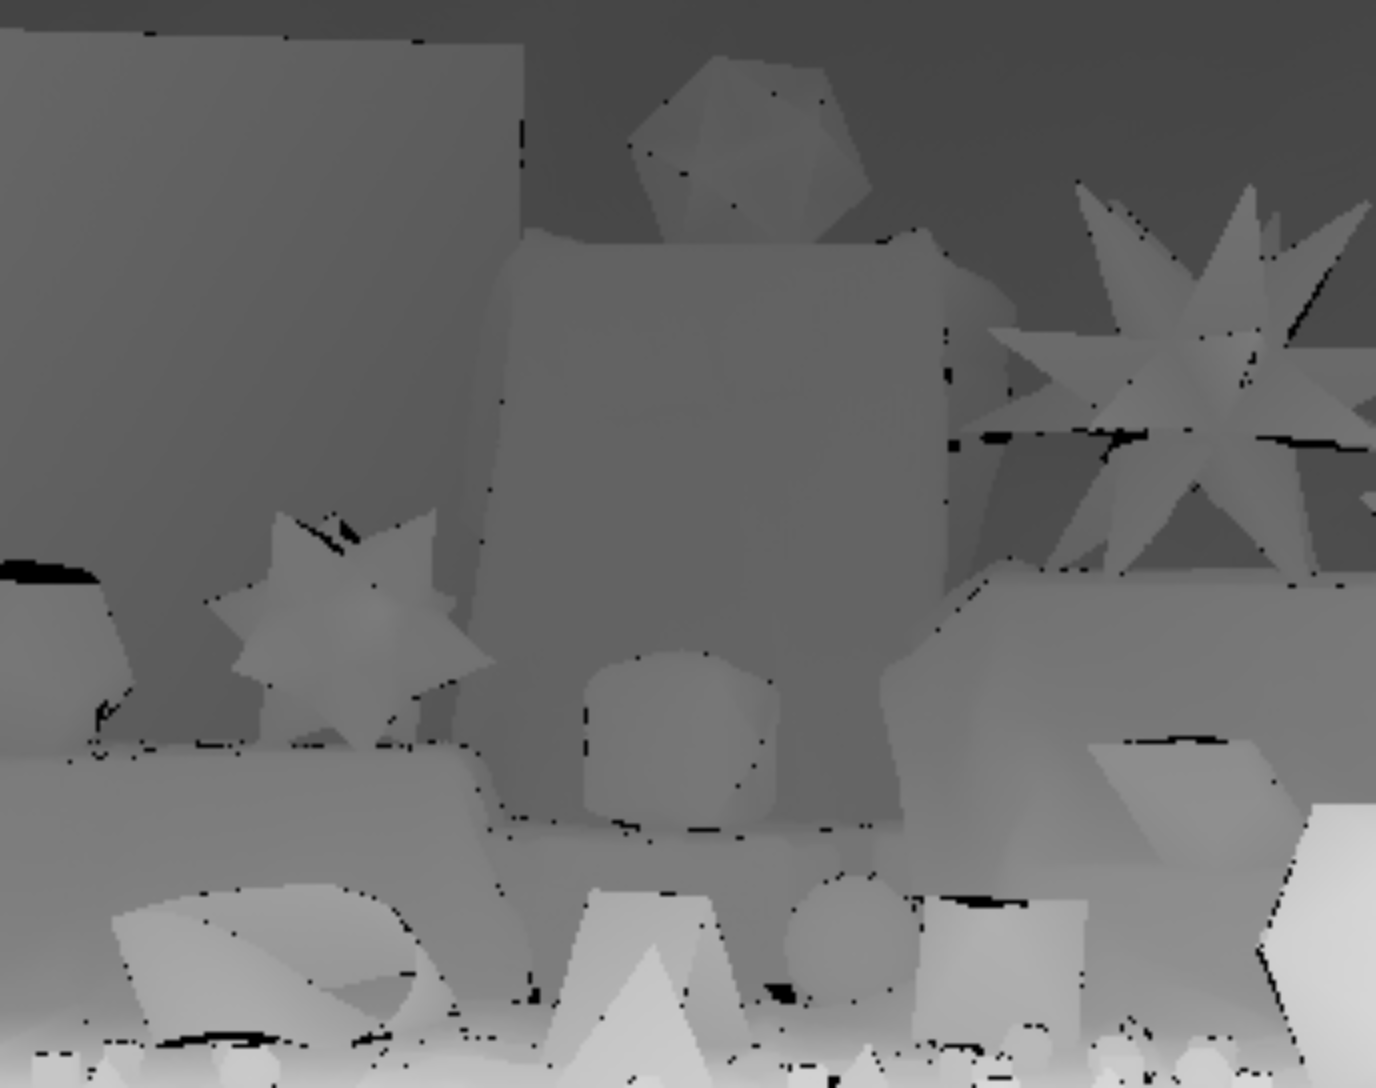
\includegraphics[width=5.5cm]{depth_interp/quan_nhf_moebius/bl.png}}
%  \vspace{1.5cm}
%   \centerline{(a)}\medskip
\end{minipage}
%
\hfill
\begin{minipage}[b]{0.48\linewidth}
  \centering
  \centerline{
\includegraphics[width=5.5cm]{depth_interp/quan_nhf_moebius/bc.png}}
%  \vspace{1.5cm}
%   \centerline{(b)}\medskip
\end{minipage}
\hfill
\begin{minipage}[b]{0.48\linewidth}
  \centering
  \centerline{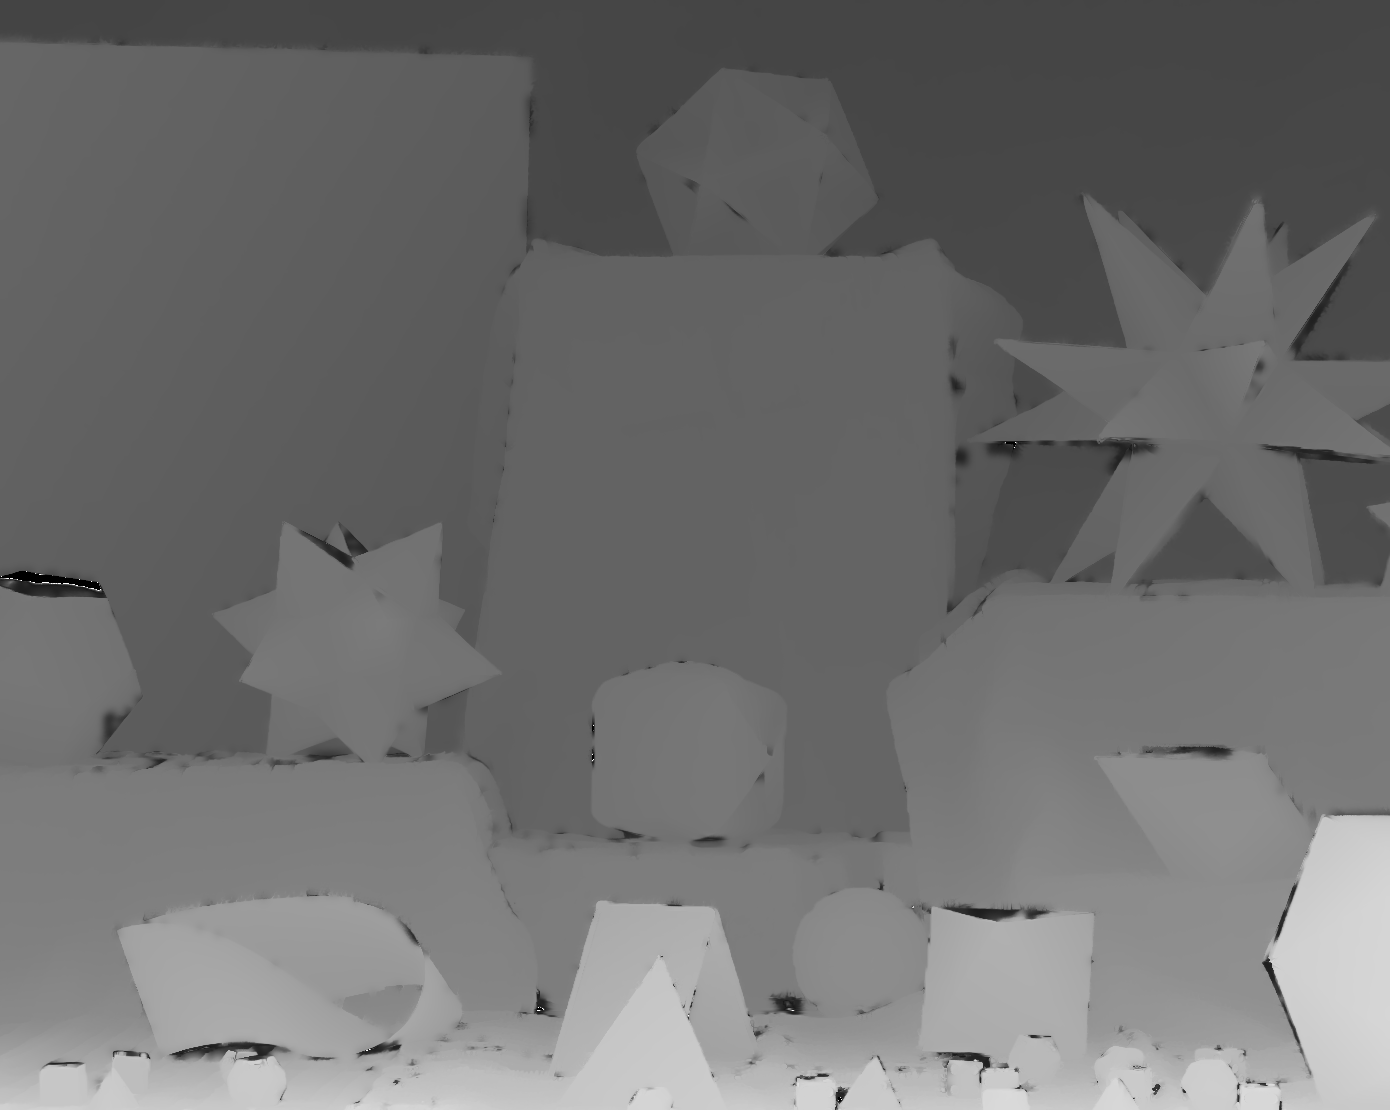
\includegraphics[width=5.5cm]{depth_interp/quan_nhf_moebius/yang.png}}
%  \vspace{1.5cm}
%   \centerline{(a)}\medskip
\end{minipage}
%
\hfill
\begin{minipage}[b]{0.48\linewidth}
  \centering
  \centerline{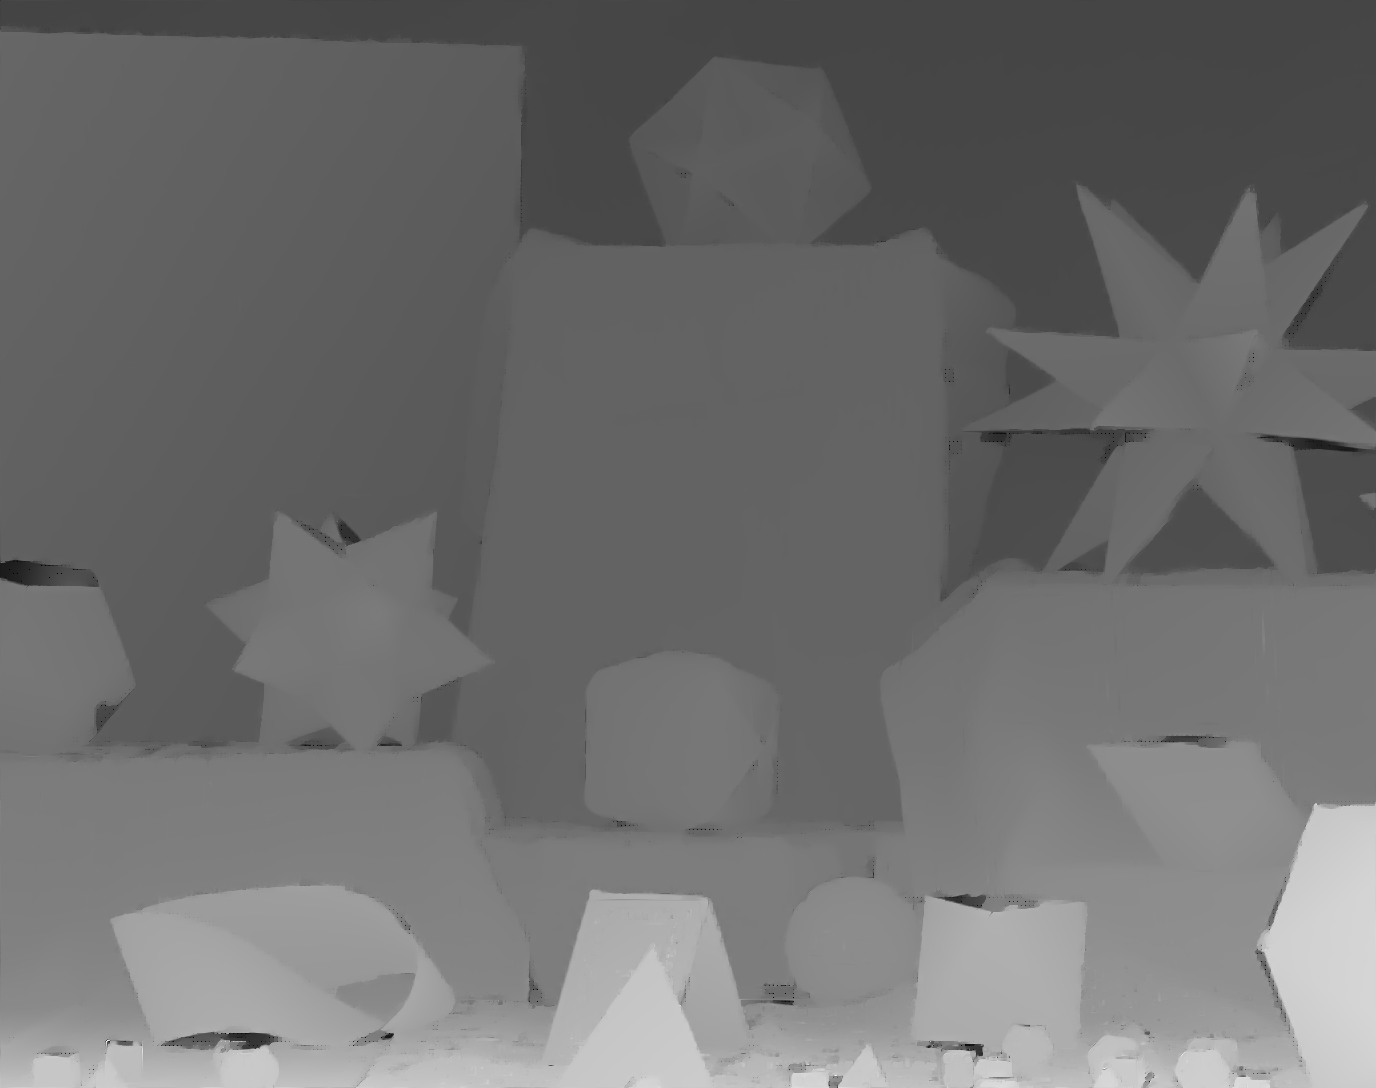
\includegraphics[width=5.5cm]{depth_interp/quan_nhf_moebius/tgv.png}}
%  \vspace{1.5cm}
%   \centerline{(a)}\medskip
\end{minipage}
%
\hfill
\begin{minipage}[b]{0.48\linewidth}
  \centering
  \centerline{\includegraphics[width=5.5cm]{depth_interp/quan_nhf_moebius/our.png}}
%  \vspace{1.5cm}
%   \centerline{(b)}\medskip
\end{minipage}
\vfill
\caption{Visual comparison of different algorithm tested on Middlebury dataset~\cite{scharstein2003high} at $4\times$ upsampling rate. Column from left to right: RGB images, ground truth, and the results of: bilinear, bicubic, IBL~\cite{yang2014color}, TGV~\cite{ferstl2013image} and proposed; row from top to bottom: Art, Books, and Moebius.}
\label{fig:quan_rst}
\end{figure*}
\begin{landscape}
\begin{table*}[t]
\centering
\resizebox{1.4\textwidth}{!}{\begin{tabular}{|c|c|c|c|c|c|c|c|c|c|c|c|c|}
\hline & \multicolumn{12}{c|}{Images}   \\ \cline{2-13} 
& \multicolumn{4}{c|}{Art}          & \multicolumn{4}{c|}{Books}        & \multicolumn{4}{c|}{Moebius}      \\ \hline
\diagbox{\tiny{Methods}}{\tiny{Sample Rate}}   &     $2\times$     & $4\times$      & $8\times$      & $16\times$     & $2\times$       & $4\times$      & $8\times$      & $16\times$     & $2\times$      & $4\times$      & $8\times$     & $16\times$    \\ \hline
bicubic                                 & 0.8965 & 1.4298 & 2.4363 & 4.3456 & 0.7911 & 1.0842 & 1.7031 & 2.5419 & 0.6855 & 1.0287 & 1.5821 & 2.5527 \\ \hline
bilinear                                & 0.7642 & 1.2300 & 2.1495 & 3.9500 & 0.6620 & 0.8993 & 1.4183 & 2.1174 & 0.5685 & 0.8578 & 1.3347 & 2.1942 \\ \hline
% MRF~\cite{diebel2005application} & --     & --     & --     & --     & --     & --     & --     & --     & --     & --     & --     & --     \\ \hline
IBL~\cite{yang2007spatial}       & 0.5016 & 0.8934 & \bf{1.7028} & 4.2324 & 0.2790 & 0.7361 & 1.4056 & 2.4561 & 0.3987 & 0.7071 & 1.1289 & 2.5885 \\ \hline
TGV~\cite{ferstl2013image}       & 0.6457 & 0.8926 & 3.2633 & 7.6490  & 0.5980 & 0.7507 & 2.3091 & 6.324  & 0.4722 & 0.5627 & 2.0375 & 6.6210  \\ \hline
Proposed                                & \bf{0.4423} & \bf{0.8765} & 1.7616 & \bf{3.6033} & \bf{0.1986} & \bf{0.3594} & \bf{0.6655} & \bf{1.1888} & \bf{0.1864} & \bf{0.3426} & \bf{0.6478} & \bf{1.2393} \\ \hline
\end{tabular}}
\caption{Quantitative comparison of different algorithms tested on Middlebury dataset~\cite{scharstein2003high}. The results is evaluated as MAE (the smaller the better) for four different sample rates, as listed in the second row. All values are computed based on the disparity maps. The best result in each situation is in bold font.}
\label{table1}
\end{table*}
\end{landscape}
% \vspace*{-0.05in}
% \subsection{Quantitative Results}

Quantitative results comparing the proposed algorithm against prior work are obtained on the Middlebury stereo dataset 2005~\cite{scharstein2003high}. We first downsample the input depth map to obtain the low resolution version, and then run different algorithms on these images to obtain the upsampled versions. We use mean absolute error (MAE) as the metric to evaluate the performance of different algorithms. Table~\ref{table1} summarizes the results\footnote{Code for IBL implementation is provided by Chunhua Shen: https://bitbucket.org/chhshen/depth-enhancement.}. Fig.~\ref{fig:quan_rst} shows the corresponding visual results at the upsampling rate of 4. The results show that our algorithm is particularly suitable for depth map upsampling, and our algorithm provides a better result compared with the other algorithms. 

%The suitability for non hole filling depth map may be more appealing considering that the real condition usually comes with many missing points. 
% In this part we show the quantitative results of our results on the Middlebury stereo dataset 2005~\cite{scharstein2003high}. We first downsample the input depth map to obtain the low resolution version, and then run different algorithms on these images to obtain the upsampled versions. We use mean absolute error (MAE) as the metric to evaluate the performance of different algorithms. Table~\ref{table1} shows the results on the original Middlebury dataset without hole filling in advance, and Table~\ref{table2} shows the results of the hole filled version provided by~\cite{park2011high}. Fig.~\ref{fig:quan_rst} shows the corresponding visual results at upsampling rate of 4. The results show that our algorithm is robust on both situation and extremely suitable for non hole filling version, which may be more appealing considering that the real condition usually comes with many missing points. In both situation, our algorithm has a result reaching the level of state of art algorithms.

% \begin{table*}[ht]
% \centering
% \resizebox{0.98\textwidth}{!}{\begin{tabular}{|c|c|c|c|c|c|c|c|c|c|c|c|c|}
% \hline & \multicolumn{12}{c|}{Images}   \\ \cline{2-13} 
% & \multicolumn{4}{c|}{Art}          & \multicolumn{4}{c|}{Books}        & \multicolumn{4}{c|}{Moebius}      \\ \hline
% \diagbox{\tiny{Methods}}{\tiny{Sample Rate}}   &     $2\times$     & $4\times$      & $8\times$      & $16\times$     & $2\times$       & $4\times$      & $8\times$      & $16\times$     & $2\times$      & $4\times$      & $8\times$     & $16\times$    \\ \hline
% bicubic           & 0.6218 & 1.0752 & 1.9778 & 3.7035 & 0.2360  & 0.3863 & 0.6732 & 1.2362 & 0.2423 & 0.3707 & 0.6645 & 1.2030 \\ \hline
% bilinear          & 0.5670 & 0.9774 & 1.8257 & 3.4853 & 0.2138  & 0.3482 & 0.6087 & 1.1290 & 0.2423 & 0.4007 & 0.7112 & 1.2715 \\ \hline
% MRF~\cite{diebel2005application}               & 0.6250 & 1.0052 & 1.9741 & 3.9370 & 0.2167  & 0.3332 & 0.6162 & 1.2107 & 0.2502 & 0.3679 & 0.6731 & 1.2884 \\ \hline
% IBL~\cite{yang2007spatial}              & 0.5709 & 0.7002 & 1.5046 & 3.6903 & 0.30130 & 0.4514 & 0.6373 & 1.4532 & 0.3868 & 0.4760 & 0.6893 & 1.1366 \\ \hline
% TGV~\cite{ferstl2013image}               & 0.5121 & 0.7842 & 2.4615 & 7.2681 & 0.2085  & 0.3470 & 1.1474 & 3.8096 & 0.1949 & 0.3221 & 1.1860 & 3.6391 \\ \hline
% Proposed              & 0.4652 & 0.9098 & 1.8183 & 3.6754 & 0.2142  & 0.3702 & 0.6688 & 1.2404 & 0.1958 & 0.3575 & 0.6674 & 1.2570 \\ \hline
% \end{tabular}}
% \caption{Quantitative comparison of different algorithms tested on Middlebury dataset with hole filled provided by~\cite{park2011high}. The results is evaluated as MAD (the smaller the better) for four different sample rates, as listed in the second row. All values are computed based on the disparity maps. The images of MRF~\cite{diebel2005application} and IBL~\cite{yang2007spatial} are provided by~\cite{park2011high}.}
% MAE (the smaller the better) of three images of the hole filled version in~\cite{park2011high}. The second row is the upsampling rate. All values are computed based on the disparity maps. The metric of MRF~\cite{diebel2005application} and IBL~\cite{yang2014color} are provided by~\cite{park2011high}}
% \label{table2}
% \end{table*}
% \begin{figure*}[ht]
% \begin{minipage}[b]{0.13\linewidth}
%   \centering
%   \centerline{\includegraphics[width=2.4cm]{quan_hf/Art.png}}
% %  \vspace{1.5cm}
% %   \centerline{(a)}\medskip
% \end{minipage}
% %
% \hfill
% \begin{minipage}[b]{0.13\linewidth}
%   \centering
%   \centerline{\includegraphics[width=2.4cm]{quan_nhf/gt.png}}
% %  \vspace{1.5cm}
% %   \centerline{(a)}\medskip
% \end{minipage}
% \hfill
% \begin{minipage}[b]{0.13\linewidth}
%   \centering
%   \centerline{\includegraphics[width=2.4cm]{quan_nhf/bl.png}}
% %  \vspace{1.5cm}
% %   \centerline{(a)}\medskip
% \end{minipage}
% %
% \hfill
% \begin{minipage}[b]{0.13\linewidth}
%   \centering
%   \centerline{\includegraphics[width=2.4cm]{quan_nhf/bc.png}}
% %  \vspace{1.5cm}
% %   \centerline{(b)}\medskip
% \end{minipage}
% \hfill
% \begin{minipage}[b]{0.13\linewidth}
%   \centering
%   \centerline{\includegraphics[width=2.4cm]{quan_nhf/yang.png}}
% %  \vspace{1.5cm}
% %   \centerline{(a)}\medskip
% \end{minipage}
% %
% \hfill
% \begin{minipage}[b]{0.13\linewidth}
%   \centering
%   \centerline{\includegraphics[width=2.4cm]{quan_nhf/tgv.png}}
% %  \vspace{1.5cm}
% %   \centerline{(a)}\medskip
% \end{minipage}
% %
% \hfill
% \begin{minipage}[b]{0.13\linewidth}
%   \centering
%   \centerline{\includegraphics[width=2.4cm]{quan_nhf/our.png}}
% %  \vspace{1.5cm}
% %   \centerline{(b)}\medskip
% \end{minipage}
% \vfill
% \begin{minipage}[b]{0.13\linewidth}
%   \centering
%   \centerline{\includegraphics[width=2.4cm]{quan_hf/gt.png}}
% %  \vspace{1.5cm}
% %   \centerline{(c)}\medskip
% \end{minipage}
% \hfill
% \begin{minipage}[b]{0.13\linewidth}
%   \centering
%   \centerline{\includegraphics[width=2.4cm]{quan_hf/bl.png}}
% %  \vspace{1.5cm}
% %   \centerline{(a)}\medskip
% \end{minipage}
% %
% \hfill
% \begin{minipage}[b]{0.13\linewidth}
%   \centering
%   \centerline{\includegraphics[width=2.4cm]{quan_hf/bc.png}}
% %  \vspace{1.5cm}
% %   \centerline{(b)}\medskip
% \end{minipage}
% \hfill
% \begin{minipage}[b]{0.13\linewidth}
%   \centering
%   \centerline{\includegraphics[width=2.4cm]{quan_hf/mrf.png}}
% %  \vspace{1.5cm}
% %   \centerline{(c)}\medskip
% \end{minipage}
% \hfill
% \begin{minipage}[b]{0.13\linewidth}
%   \centering
%   \centerline{\includegraphics[width=2.4cm]{quan_hf/yang.png}}
% %  \vspace{1.5cm}
% %   \centerline{(a)}\medskip
% \end{minipage}
% %
% \hfill
% \begin{minipage}[b]{0.13\linewidth}
%   \centering
%   \centerline{\includegraphics[width=2.4cm]{quan_hf/tgv.png}}
% %  \vspace{1.5cm}
% %   \centerline{(a)}\medskip
% \end{minipage}
% %
% \hfill
% \begin{minipage}[b]{0.13\linewidth}
%   \centering
%   \centerline{\includegraphics[width=2.4cm]{quan_hf/our.png}}
% %  \vspace{1.5cm}
% %   \centerline{(b)}\medskip
% \end{minipage}
% \vfill
% \caption{Visual comparison of different algorithm tested on Middlebury dataset~\cite{scharstein2003high} at $4\times$ upsampling rate. Top from left to right: RGB image of Art, non hole filled ground truth, and the results of: bilinear, bicubic, IBL~\cite{yang2014color}, TGV~\cite{ferstl2013image} and ours; bottom from left tot right: hole filled ground truth~\cite{park2011high}, and the results of: bilinear, bicubic, MRF~\cite{diebel2005application}, IBL~\cite{yang2014color}, TGV~\cite{ferstl2013image} and ours.}
% \label{fig:quan_rst}
% \end{figure*}

\subsection{Discussion}
\label{sec:2.discussion}
%The proposed algorithm is based on the assumption that for a small patch, the depth values are linear in the spatial coordinates and the edges on depth map are controlled by the corresponding RGB image. 
Table~\ref{table1} illustrates that the depth map upsampling obtained with the proposed algorithm is accurate and achieves the state of the art results on the common benchmarking dataset, providing a better performance compared with other algorithms. The proposed algorithm, however, still suffers from two limitations. First, there are a few outlier points where the method yields a large error. Second, the edges are not sharply defined, especially under high upsampling rate, which is typical in most depth upsampling algorithms. The computational requirements are an additional challenge: to process a $1088\times 1296$ pixel image, our algorithm takes about 40min. While the time requirement is analogous for several other upsampling algorithms, a speed-up is desirable for many applications. 

We also want to mention more about the relation of the proposed algorithm with Levin's~\cite{levin2008closed} matting method and He's~\cite{he2010fast} fast computing algorithm. Levin's method is to formulate a linear combination of neighbour pixels value for estimating matting map, or alpha channel; He's method is based on Levin's formulation and proposed the acceleration also using conjugate gradient. In our problem, we utilize the linear relation of spacial instead direct pixel values; and, we formulate a local filtered conjugate gradient formulation using conjugate gradient, instead of an adjacent matrix. The similarity and difference of the proposed algorithm with Levin's method is listed in~\ref{table:relation_matting}.  

\begin{table}[htb]
\centering
\resizebox{0.98\textwidth}{!}{
\begin{tabular}[c]{l|l|l}
 & Levin's matting method    & Proposed method
 \\ \hline
similarity & \multicolumn{2}{l}{\begin{tabular}{l}\tabitem linear model\\
\tabitem build Laplacian matrix to solve the optimization\end{tabular}}           \\ \hline
difference & linear in color intensity & \begin{tabular}{l} \tabitem linear in relative spatial location\\ \tabitem weight based on color information\end{tabular}
\end{tabular}}
\caption{Similarity and difference of the proposed algorithm with Levin's method~\cite{levin2008closed.}}
\label{table:relation_matting}
\end{table}

%the challenging because it is both application and content dependent.

% Our algorithm is based on the assumption that in a small patch, the depth values are linear and the edges on depth map are controlled by the corresponding RGB image. From Table~\ref{table1} and Table~\ref{table2} we find that the depth map upsampling is accurate at low upsampling rate and achieves the state of the art results on the common benchmarking dataset. Meanwhile, through the comparison of the two tables, our algorithm proves a better performance on non hole filling version which may be more accustomed to actual usage. However, this algorithm still suffers from two problems. First, there are some bad point with very low disparity value after the interpolation. Second, the edge, especially under high upsampling rate, is not satisfying, which is typical in most depth upsampling algorithms. Meanwhile, to process an image with resolution $1088\times 1296$, our algorithm takes about 40min, which is time consuming as many other depth upsampling algorithms. In our future work, we aim at alleviating these problems by implementing some post processing using segmentation techniques, and use techniques such as a coarse to fine structure~\cite{Chao:Colorization:pspie9020} to accelerate the computing.

\section{Conclusion}
\label{sec:2.conclusion}
%In this paper we propose a novel algorithm for both low resolution depth map upsampling and high resolution depth map hole filling. 

The algorithm proposed in this paper provides an effective method for depth map upsampling and hole filling. Quantitative results on test data indicates that the method offers an improvement over current state of the art methods and visual assessment shows that the depth map estimated by the proposed technique is consistent with the color images.

% Compared to several the state of the art, our proposed algorithm offers improved accuracy

%Our algorithm assumes a linear relation in patches of the depth map, and optimizes an objective constructed on the weighted linear fitting. We showed the qualitative and quantitative experiments of our algorithm and the comparison with other algorithms. The result shows that our algorithm reach the level of state of art algorithms and extremely suitable for depth map upsampling with many missing points.

%%% Local Variables: 
%%% mode: latex
%%% TeX-master: "dissertation"
%%% End: 
\setcounter{section}{0}
\let\oldthesection\thesection
\renewcommand{\thesection}{\thechapter.\Alph{section}}
\section{Appendix to Chapter~\ref{sec2.3.2}}
\label{ap1}
For ~\eqref{eq:2.6},
\begin{equation}
\begin{split}
P_{j} &=  {\argmin}_{P_{j}}{((W_{j}(D_{H,N_{j}}-GP_{j}^T))^2)}\\
&= (G^{T}W_{0,j}^{T}G)^{-1}G^{T}W_{0,j}^{T}D_{H,N_{j}},
\end{split}
\end{equation}
so,
\begin{equation}
\begin{split}
d((W_{j}(D_{H,N_{j}}-GP_{j}^T))^2)/dP_{j} &= 0\\
&= W_{j}(D_{H,N_{j}}-GP_{j}^T))G^T,
\end{split}
\end{equation}
solve the linear equation gives,
\begin{equation}
P_{j} = (G^{T}W_{0,j}^{T}G)^{-1}G^{T}W_{0,j}^{T}D_{H,N_{j}}.
\end{equation}

For ~\eqref{eq:2.7},
\begin{equation}
\begin{split}
Q &= \sum_{j=1}^{N}{(W_{j}(D_{H,N_{j}}-G{(G^{T}W_{0,j}^{T}G)^{-1}G^{T}W_{0,j}^{T}D_{H,N_{j}}}^T))^2+{\lambda}F_{j}}\\
&= \sum_{j=1}^{N}{((W_{j}D_{H,N_{j}})(E-G{(G^{T}W_{0,j}^{T}G)^{-1}G^{T}W_{0,j}^{T}}^T))^2+{\lambda}F_{j}}\\
&= \sum_{j=1}^{N}{D_{H,N_{j}}^{T}(\overline{G_{j}}^{T}W_{0,j}\overline{G_{j}})D_{H,N_{j}}}+{\lambda}F_{j}\\
&= \sum_{j=1}^{N}{D_{H,N_{j}}^{T}(\overline{G_{j}}^{T}W_{0,j}\overline{G_{j}})D_{H,N_{j}}}+\sum_{j=1}^{M}{\lambda(D_{L,j}-D_{H,j})^2},
\end{split}
\label{eq:2.7}
\end{equation}


\renewcommand{\thesection}{\thechapter.\Alph{section}}
\section{Appendix to Chapter~\ref{sec2.3.3}}
\label{ap2}
For~\eqref{eq:2.cgs_final},
\begin{equation}
\begin{split}
(Lp)_{i} &= \sum{\delta_{ij}w_{ki}P_{i}}-G_{i}\sum_{k\in N_{i}}{a_{k}w_{ki}}+\sum_{k\in N_{i}}{b_{k}w_{ki}}\\
&= \sum{\delta_{ij}w_{ki}P_{i}}-G_{i}\sum_{k\in N_{i}}{a_{k}w_{ki}k_{0}a_{k}w_{ki}}\\
&= \sum{\delta_{ij}w_{ki}P_{i}}-G_{i}\sum_{k\in N_{i}}{(C_{k}(\sum_{j\in N_{k}}{w_{kj}}G_{j}P_{j}-k\overline{p_{k}}))w_{ki}k_{0}a_{k}w_{ki}}\\
& = \sum_{j}{(\sum_{k|i,j\in N_{k}}{(\delta_{ij}w_{ki}-w_{ki}w_{kj}(G_{i}-k_{0})C_{k}(G_{j}-k_{0}))})p_j},
\end{split}
\end{equation}
which demonstrates the consistency of two different expression.
% Go back to the old section numbering for future chapters
\let\thesection\oldthesection
\chapter{Hazerd: an outdoor scene dataset and benchmark for Single image dehazing}
\label{cha3}
\chaptermark{Hazerd: a dehazing dataset and benchmark}

\section{Introduction}
\label{sec:3.1.intro}
Haze is a common degradation encountered in outdoor images, where image contrast is reduced due to light scattered by particles suspended in the air. Koschmieder~\cite{Koschmieder24,McCartney76} proposed a classical physical model to explain haze, in which horizontal airlight from scattering and light reflected by objects, transmitted and attenuated in the propagation through the hazy air, both contribute to the final images and the ratio of their contributions are controlled by the optical thickness of the media between the camera sensor and the object being imaged. The loss of detail caused by haze makes images aesthetically unappealing and also poses challenges for both human and machine vision, making it difficult to recognize and track objects and to navigate.

To mitigate the impact of haze, physics-based algorithms have been proposed for haze removal or {\em dehazing}. Early works mainly focus on image dehazing utilizing additional information. Such works includes: in~\cite{narasimhan2003contrast}, two images under different weather conditions for the same location are exploited for haze removal; in~\cite{kopf2008deep}, rough geological information is used; and in~\cite{schaul2009color}, the fusion  of near-infrared images and the hazy images are utilized for enhancing the details. These algorithms need multiple images or additional information. Though proved to be efficient, these works need either multiple images or information other than RGB images, which may be inaccessible for general applications, for example outdoor image dehazing taken by mainstream consumer-level digital cameras.

In this chapter we focus on single image dehazing methods that typically seek to estimate both the airlight and the transmission from a single hazy image, which is an ill-posed problem. To address the ill-posedness most algorithms impose additional constraints or assumptions to obtain solutions. In~\cite{fattal2008single,fattal2014dehazing,berman2016non}, color-line or haze-line has been used for modeling the spatial variance of similar color objects. In~\cite{tarel2009fast}, constraints on air veil are imposed based on the physical model. In~\cite{tan2008visibility}, the assumption of higher contrast and local smoothness are introduced. In~\cite{he2011single}, a dark channel prior is proposed that postulates that the color channel with lowest intensity represents airlight. The dark prior is extended in~\cite{meng2013efficient} to accommodate color boundary constraints. An alternative color attenuation prior is used with supervised learning in~\cite{zhu2015fast} and image fusion based approaches are proposed in~\cite{ancuti2010fast,ancuti2013single}.
In~\cite{nishino2012bayesian}, a Bayesian framework for haze estimation is described. In~\cite{cai2016dehazenet, Ren-ECCV-2016}, deep learning networks are designed for estimating the transmission map.

Despite the large number of algorithms proposed for single image dehazing, there are no established criteria or metrics for their evaluation and past publications have primarily relied on subjective comparisons on a limited number of images, with different publications using different sets of images. Three datasets: FRIDA~\cite{tarel2012vision}, D-hazy~\cite{7532754}, and CHIC~\cite{el2016color} have been proposed in prior work for objective evaluation of algorithms. FRIDA~\cite{tarel2012vision} is rather specialized and provides several synthetic hazy road images from a driver's viewpoint. D-hazy uses depth images from the Middlebury~\cite{scharstein2014high} and the NYU depth V2~\cite{silberman2012indoor} which are indoor scenes not representative of the typical dehazing applications. CHIC uses a fog machine in an indoor environment and provides 2 indoor scenes with known objects (e.g. Macbeth color checker) and 2 scenes that include outdoor content seen through windows. The indoor fog generation makes these images atypical, particularly for the case where an outdoor haze-free scene is seen from haze within the room.

In this
chapter, we provide a new image dataset {\em HazeRD}, {\em Haze Realistic Dataset}, for benchmarking of dehazing algorithms that consists of ten different actual outdoor scenes at high resolution with simulated haze under five different weather conditions, where realistic parameter values are chosen based on scattering theory. As compared to the indoor scenes used in~\cite{7532754}, these scenes are more representative of the outdoor conditions under which dehazing is of interest and they correspond to actual images as opposed to the synthetically generated versions in~\cite{tarel2012vision}. We benchmark a number of single image dehazing algorithms both on the proposed new dataset and on the existing D-hazy dataset~\cite{7532754}. Our results demonstrate that there are significant differences between the performance of the different algorithms on different datasets and the rank order of algorithms is by no means constant over the different datasets, thereby emphasizing the need for datasets like ours that are matched with realistic conditions under which dehazing is utilized.

The chapter is organized as follows. Section~\ref{sec:3.2.model} discusses the physical model for atmosphere scattering and image formation; Section~\ref{sec:3.3.simu} describes the simulation process; Section~\ref{sec:3.4.dataset} discusses the HazeRD dataset; Section~\ref{sec:3.5.benchmark} briefly summarizes some state of art dehazing techniques and their performance; at last, Section~\ref{sec:3.6.discussion}, discusses some noteworthy points about dehazing problems and the future work that may be done with HazeRD.

\section{physical model for haze}
\label{sec:3.2.model}
Atmospheric optics interprets the propagation of light in haze or fog as the process of light random diffusion and reflection by the particles in the air. Hazy weather is caused by the particles, mainly water droplets distributed in the air, which vary in both the size and the density. Haze, fog and cloud in principle share the same components, namely the air with multiple sized water droplets, but differ in the average size and distribution. The scattering of single water droplet has different behaviours regarding to the size, or the radius of the droplet: Rayleigh scattering deals with conditions that the radius is of the size of visible light wavelengths, which corresponding to almost clear weather; and Mie scattering deals with those with the radius far beyond the wavelengths, which displays high anisotrophy in the scattered light. The accumulated contribution of the distribution of the water droplets ultimately form the scattered light of the incident light. Table~\ref{table:hazelvl} lists different weather and the corresponding particles making the main contribution.
\begin{figure}[t]
\centering
\centerline{\includegraphics[width=0.95\columnwidth]{hazerd/physical_model.jpg}}
\caption{The physical model for haze. Light at the sensor is composed of airlight scattered by particles suspended in the air and light reflected from imaged objects, which is attenuated when propagating through the air.}
\label{fig:3.2.physical}
\end{figure}

\begin{table}[t]
\centering
\resizebox{0.8\textwidth}{!}{\begin{tabular}{l|l|l}
Type           & Radius($\mu m$)                                    & Concentration($cm^-3$)          \\\hline
Air molecule   & $10^{-4}$ & $10^{19}$ \\
Aitken nucleus & $10^{-4}$-$10^{-2}$ & $10^4$-$10^2$       \\
Haze Particle  & $10^{-2}$-$1$                     & $10^2$-$1$ \\
Fog droplet    & 1-10                                          & 100-10                                          \\
Cloud droplet  & 1-10                                          & 300-10                                          \\
Raindrop       & $10^2$-$10^4$     & $10^{-2}$-$10^{-5}$
\end{tabular}}
\caption{Particle sizes for different weather}
\label{table:hazelvl}
\end{table}

As refer to above, Mie scattering theory~\cite[Chap. 5, 6]{McCartney76}, which applies when particle sizes are significantly larger that the wavelengths of light involved, can be used to analyze light propagation under hazy conditions. While the exact details of Mie theory are quite involved, image formation under hazy weather can be modeled by taking two main factors into account: the airlight and the attenuation. The physical scenario is depicted in Fig.~\ref{fig:3.2.physical}. Due to the scattering of light by the particles in the haze, light from objects attenuates as it propagates from the object to the camera with an intensity that declines exponentially with distance. At the same time, part of the ambient illumination is scattered by the haze particles into the camera as {\em airlight} that increases the intensity of the image.  Assuming a homogeneous haze and a uniform ambient illumination, the spectral irradiance incident on the camera sensor plane from an object with spatially uniform spectral irradiance $E_{\lambda}$  can be written as~\cite{Koschmieder24},
\begin{equation}
I_{\lambda} = t_{\lambda} E_{\lambda} + (1-t_{\lambda})A_{\lambda},
\label{eq:3.1}
\end{equation}
where $\lambda$ denotes the wavelength,  $A_{\lambda}$ is the {\em airlight}, and $t_{\lambda} = e^{-d \beta{_\lambda}}$ is the so called {\em transmission}, with $\beta{_\lambda}$  denoting the scattering coefficient for the haze particles, and $d$ denoting the distance between the object and the camera. The product $d \beta{_\lambda}$ is called the {\em optical thickness}. Observe that as the distance $d$ increases, the contribution of airlight increases while the light from the object diminishes, leading to reduced contrast. The image captured by a typical three channel RGB (red-green-blue) camera can then be expressed as,
\begin{equation}
% \begin{aligned}
% I_{C} &= \int_{\lambda}{I_{\lambda}*R_{\lambda,C}}d\lambda \\
%  &= \int_{\lambda}{t_{\lambda}*E_{\lambda}*R_{\lambda,C}+(1-t_{\lambda})*A_{\lambda}*R_{\lambda,C}}d\lambda,
% \end{aligned}
I_{C} = \int_{\lambda}{t_{\lambda} E_{\lambda} R_{\lambda,C}+(1-t_{\lambda}) A_{\lambda} R_{\lambda,C}}d\lambda,
\label{eq:3.2}
\end{equation} 
where $C\in{\{R,G,B\}}$ represents the image channel and $R_{\lambda,C}$ the camera spectral response of the channel.

\section{Haze simulation}
\label{sec:3.3.simu}
In dense haze or fog, the scattering coefficient $\beta_{\lambda}$ is almost constant over the visible spectral region, and therefore we can simplify~\eqref{eq:3.2} by setting $\beta_{\lambda} = \beta$ for all wavelengths $\lambda$. The captured image channel intensities can then be represented as 
% Following the idea in~\cite{blasinski2013per}, in which the value of each channel is dealt with separately and pixel-wise, the relation for hazy image simulation in position $(x,y)$ is,
\begin{equation}
I_{C}(x,y) = E_{C}(x,y) t(x,y) +A_{C}(x,y) (1-t(x,y)),
\label{eq:3.3}
\end{equation}
\begin{equation*}
t(x,y) = e^{-\beta d(x,y)},
\end{equation*}
% \vspace*{-0.06in}
% \begin{align*}
% E_{C}(x,y) &= \int_{\lambda}{E_{\lambda}(x,y) R_{\lambda,C}}d\lambda,\\
% A_{C} &= \int_{\lambda}{A_{\lambda}R_{\lambda,C}}d\lambda,
% \vspace*{-0.05in}
% &\end{align*}
where $(x,y)$ denotes spatial location, 
%$E_{C}(x,y) = \int_{\lambda}{E_{\lambda}(x,y) R_{\lambda,C}}d\lambda$
\[
E_{C}(x,y) = \int_{\lambda}{E_{\lambda}(x,y) R_{\lambda,C}}d\lambda,
\]
is the irradiance of the object received by camera sensor in the absence of haze, i.e., the haze-free image, and $A_{C} = \int_{\lambda}{A_{\lambda}R_{\lambda,C}}d\lambda$ is the airlight, and the depth $d(x,y)$ denotes the distance of the object imaged at $(x,y)$ from the camera plane. Note that a key advantage of the simplified model is that hazy images can be simulated using only haze free images along with depth information using the scattering parameter $\beta$ and the airlight $A_{C}$ and the spectral distributions on the right hand side of~\eqref{eq:3.2}, which are invariably unavailable, are not required for the haze simulation. The color and gamma correction~\cite{GSharma:crcdcihbk02} in encoding the raw camera sensor values into digital images, however, need to be accounted for. Images are typically encoded in the 
sRGB color space~\cite{international1999multimedia}. We assume that the color correction matrix is absorbed into the channel sensitivities in~\eqref{eq:3.2} and the "linear" intensity values from~\eqref{eq:3.3} are nonlinearly encoded into the digital image values via the transform specified in the sRGB standard~\cite{international1999multimedia}, viz.,
\begin{equation}
C = \begin{cases}
12.92C_{L} &\text{C $\le$ 0.0031308},\\
1.055C_{L}^{1/2.4}-0.055 &\text{C $>$ 0.0031308},
\end{cases}
\label{eq:3.srgb2rgb}
\end{equation}
here $C_{L}$ is the linear RGB value for each channel, $C$ is the corresponding sRGB encoded value, where the transformation is specified on a $[0-1]$ range which is then mapped to the 8-bit digital encoding. For the simulation, the inverse of the transformation in~\eqref{eq:3.srgb2rgb} is applied to the recorded haze free image after mapping the data into the  $[0-1]$ range and once the simulated hazy images are obtained via~\eqref{eq:3.3} the transformation in~\eqref{eq:3.srgb2rgb} is applied and the images are re-encoded as 8-bit representations.

%We use visual range to describe the weather condition. 
The scattering parameter $\beta$ depends on the weather conditions. Its value is specified in terms of the intuitive notion of visual range~\cite[pp. 42]{McCartney76}, which is defined, under daylight conditions, as the distance at which the apparent contrast between a dark object and the horizon sky becomes equal to the just noticeable contrast threshold $\epsilon$ for an observer (usually set to 0.02). Specifically, the scattering parameter is obtained from the visible range $R_{m}$ via the relation $\beta = -\ln(\epsilon)/R_m $. HazeRD simulates five different conditions from light to dense fog, for which the visible range and the scattering parameter are listed in Table.~\ref{table:3.coefficient}. For simulating hazy images, HazeRD uses~\eqref{eq:3.3} with these parameter values along with captured haze free images that also have an associated depth map $d(x,y)$ available. Fig.~\ref{fig:3.simu} summarizes the the haze simulation process.

% \vspace*{-0.1in}
% \begin{equation}
% \beta = \frac{1}{R{_m}}\ln\frac{1}{\epsilon},
% \label{eq:4}
% \vspace*{-0.05in}
% \end{equation}
\begin{table}[htp]
\centering
\resizebox{0.95\textwidth}{!}{\begin{tabular}{|c|c|c|c|c|c|c|} \hline
 & 50m & 100m & 200m & 500m & 1000m \\ \hline
weather condition & dense & thick & thick & moderate & light \\ \hline
scattering coef. $\beta$ & 78.2 & 39.1 & 19.6 & 7.82 & 3.91  \\ \hline
\end{tabular}}
\caption{The visual range in HazeRD, and the corresponding weather condition and the scattering coefficient $\beta$.}
\label{table:3.coefficient}
\end{table}
\begin{figure}
\centering
\centerline{\includegraphics[width = 0.95\linewidth]{hazerd/simulation}}
\caption{Flow for haze simulation based on~\eqref{eq:3.3}.}
% TBD: Yanfu, please move the E_c(x,y) to clearly indicate that that is in the linear space
\label{fig:3.simu}
\end{figure}

% As mentioned before, the relation only holds true for visible light. In the infrared waveband, the scattering coefficient may not be viewed as constant. For example, at the wavelength of 3.61um with the visual range of 3.55km, the transmission is still as high as 0.72, whereas in the visible waveband it is only 0.1~\cite{McCartney76}. This indicates the potential of exploiting the infrared information in image dehazing or enhancement.
\section{dataset}
\label{sec:3.4.dataset}
For performance of single image dehazing algorithms, HazeRD provides ten scenes, each one having a clean RGB image and a ground truth depth map. The dataset is derived from the architectural biometrics project~\cite{Ding:ArchBio:ICIP16,ArchBioProjWebsite}, on which we first estimate the dense depth maps for each scene by fusing structure from motion and lidar~\cite{Ding:FuseLidarSFM:ICASSP17}. Five different weather conditions are simulated in each scene, ranging from light fog to dense fog, in order to test the robustness of dehazing algorithms. See Fig.~\ref{fig:3.block_diagram} for the dataset generation and benchmark block diagram. The simulation of haze and fog is performed by inverse application of ~\eqref{eq:3.srgb2rgb} followed by ~\eqref{eq:3.3}, re-white balance and redo the gamma correction. The color image values are converted to $[0,1]$ for implementing the color space transferring. Then, we use a weighted median filter~\cite{ma2013constant} and the triangular interpolation for the refinement of the depth map. The airlight is set to 0.86, to ensure a visual vividness of objects in overcast weather. Sky area, where typically depth values are missing, is set to have the distance of two times the visual range, which ensures that the transmission is of the order $10^{-4}$ and that almost no noise is introduced for normal pictures. A sample of hazy images derived from one of the original images in HazeRD is shown in Fig.~\ref{fig:3.example_dataset} for a number of different visual ranges. Figure.~\ref{fig:3.hist_compare} shows the depth histograms of HazeRD and for the Middlebury and NYU datasets that also provide images and depth maps required for haze simulation. Compared to the other two datasets which focus primarily on indoor images, the outdoor images in HazeRD span a much larger range of distance ranges and show clear clustering of different object depths. For each scene and the weather condition, a noisy version is provided. Considering the complexity of the real environment, strictly homogeneity is impossible. In atmospheric optics the main component of random fluctuations usually can be expressed by low-order Seidel aberration; here we use the Perlin noise to simulate this phenomenon~\cite{tarel2012vision}. 
\begin{figure}[htb]
% \setlength{\textfloatsep} {0pt plus 2pt minus 2pt}
% \setlength\abovecaptionskip{0pt}
% \setlength\belowcaptionskip{0pt}
\centering
\centerline{\includegraphics[width = 0.95\textwidth]{hazerd/block_diagram}}
\caption{Benchmarking workflow for evaluating dehazing algorithms using the HazeRD(proposed) and D-Hazy~\cite{7532754} dataset.}
\label{fig:3.block_diagram}
\end{figure}
\begin{figure}[htb]
\begin{minipage}[b]{0.24\linewidth}
  \centering
  \centerline{\includegraphics[width=3.2cm]{hazerd/dataset/IMG_8612_50}}
%  \vspace{1.5cm}
%   \centerline{(a)}\medskip
\end{minipage}
%
\hfill
\begin{minipage}[b]{0.24\linewidth}
  \centering
  \centerline{\includegraphics[width=3.2cm]{hazerd/dataset/IMG_8612_100}}
%  \vspace{1.5cm}
%   \centerline{(b)}\medskip
\end{minipage}
\hfill
\begin{minipage}[b]{0.24\linewidth}
  \centering
  \centerline{\includegraphics[width=3.2cm]{hazerd/dataset/IMG_8612_200}}
%  \vspace{1.5cm}
%   \centerline{(c)}\medskip
\end{minipage}
\begin{minipage}[b]{0.24\linewidth}
  \centering
  \centerline{\includegraphics[width=3.2cm]{hazerd/dataset/IMG_8612_500}}
%  \vspace{1.5cm}
%   \centerline{(d)}\medskip
\end{minipage}
\caption{HazeRD Samples. From left to right: a hazy image, with the visual range of 50m, 100m, 200m, and 500m respectively.}
\label{fig:3.example_dataset}
\end{figure}
\begin{figure}[htb]
\centering
\resizebox{0.95\textwidth}{!}{
\begin{minipage}[b]{0.54\linewidth}
  \centering \centerline{\includegraphics[width=9cm]{hazerd/hist/hist_all}}
%   \centerline{(a)}\medskip
 \end{minipage}
\begin{minipage}[b]{0.44\linewidth}
  \centering \centerline{\includegraphics[width=5.5cm]{hazerd/hist/hist_mn}}
%   \centerline{(b)}\medskip
 \end{minipage}}
\caption{Histograms of 3 dataset. Left: HazeRD, Middlebury, and NYU, right: the Middlebury dataset and NYU.}
\label{fig:3.hist_compare}
\end{figure}

\section{benchmark: algorithms and datasets}
\label{sec:3.5.benchmark}
As mentioned above, a typical dehazing algorithm usually has two stages: first, some priors or constraints are formulated to regularize the underconstrained problem, then a loss function is minimized to determine a solution; which is then refined using the hazy images, mainly to eliminate halos or artificial details. In this section, we benchmark six state of art dehazing algorithms described in the following, which we referred to by the labels corresponding to the first author's last name as: (1) He~\cite{he2011single}, (2) Meng~\cite{meng2013efficient}, (3) Zhu~\cite{zhu2015fast}, (4) Berman~\cite{berman2016non}, (5) Cai~\cite{cai2016dehazenet} and (6) Ren~\cite{Ren-ECCV-2016}.
% \begin{itemize}
%     \item He~\cite{he2011single}
%     \item Meng~\cite{meng2013efficient}
%     \item Zhu~\cite{zhu2015fast}
%     \item Berman~\cite{berman2016non}
%     \item Cai~\cite{cai2016dehazenet}
% \end{itemize}
% We briefly summarize the algorithms in order to subsequently understand their success and failure. Some examples of these techniques on HazeRD and synthesized NYU and Middlebury dataset are showed in Fig.~\ref{fig:exmaple_3dpc} and Fig.~\ref{fig:exmaple_nyu_middlebury}.
We briefly summarize the algorithms in order to subsequently understand their success and failure. Some examples of these techniques on HazeRD and synthesized NYU and Middlebury dataset are showed in Fig.~\ref{fig:3.exmaple.hazerd}, Fig.~\ref{fig:3.exmaple.hazerd.trans}, Fig.~\ref{fig:3.exmaple.nyu}, and Fig.~\ref{fig:3.exmaple.middlebury}.
\begin{figure*}[htb]
\begin{subfigure}[b]{1\linewidth}
  \centering
  \centerline{\includegraphics[width=6cm]{hazerd/img/ori_img}}
  \subcaption{}
\end{subfigure}
\vfill
\begin{subfigure}[b]{0.45\linewidth}
  \centering
  \centerline{\includegraphics[width=5cm]{hazerd/img/dehaze_he}}
  \subcaption{}
\end{subfigure}
\hfill
\begin{subfigure}[b]{0.45\linewidth}
  \centering
  \centerline{\includegraphics[width=5cm]{hazerd/img/dehaze_meng}}
  \subcaption{}
\end{subfigure}
\vfill
\begin{subfigure}[b]{0.45\linewidth}
  \centering
  \centerline{\includegraphics[width=5cm]{hazerd/img/dehaze_zhu}}
  \subcaption{}
\end{subfigure}
\hfill
\begin{subfigure}[b]{0.45\linewidth}
  \centering
  \centerline{\includegraphics[width=5cm]{hazerd/img/dehaze_berman}}
  \subcaption{}
\end{subfigure}
\vfill
\begin{subfigure}[b]{0.45\linewidth}
  \centering
  \centerline{\includegraphics[width=5cm]{hazerd/img/dehaze_cai}}
  \subcaption{}
\end{subfigure}
\hfill
\begin{subfigure}[b]{0.45\linewidth}
  \centering
  \centerline{\includegraphics[width=5cm]{hazerd/img/dehaze_ren}}
  \subcaption{}
\end{subfigure}
\vfill
\caption{Example of algorithms' performances. (a): a haze free image from HazeRD, and the results of dehazing of a corresponding hazy image obtained with: (b):He~\cite{he2011single}, (c): Meng~\cite{meng2013efficient}, (d): Zhu~\cite{zhu2015fast}, (e): Berman~\cite{berman2016non}, (f): Cai~\cite{cai2016dehazenet}, and (g): Ren~\cite{Ren-ECCV-2016}.}
\label{fig:3.exmaple.hazerd}
\end{figure*}
\begin{figure*}[htb]
\begin{subfigure}[b]{1\linewidth}
  \centering
  \centerline{\includegraphics[width=6cm]{hazerd/img/ori}}
  \subcaption{}
\end{subfigure}
\vfill
\begin{subfigure}[b]{0.45\linewidth}
  \centering
  \centerline{\includegraphics[width=5cm]{hazerd/img/he}}
  \subcaption{}
\end{subfigure}
\hfill
\begin{subfigure}[b]{0.45\linewidth}
  \centering
  \centerline{\includegraphics[width=5cm]{hazerd/img/meng}}
  \subcaption{}
\end{subfigure}
\vfill
\begin{subfigure}[b]{0.45\linewidth}
  \centering
  \centerline{\includegraphics[width=5cm]{hazerd/img/zhu}}
  \subcaption{}
\end{subfigure}
\hfill
\begin{subfigure}[b]{0.45\linewidth}
  \centering
  \centerline{\includegraphics[width=5cm]{hazerd/img/berman}}
  \subcaption{}
\end{subfigure}
\vfill
\begin{subfigure}[b]{0.45\linewidth}
  \centering
  \centerline{\includegraphics[width=5cm]{hazerd/img/cai}}
  \subcaption{}
\end{subfigure}
\hfill
\begin{subfigure}[b]{0.45\linewidth}
  \centering
  \centerline{\includegraphics[width=5cm]{hazerd/img/ren}}
  \subcaption{}
\end{subfigure}
\vfill
\caption{Example of algorithms' performances. (a): the ground truth transmission for the haze free image in~\ref{fig:3.exmaple.hazerd}, and the transmission estimates corresponding to the estimated images obtained with: (b):He~\cite{he2011single}, (c): Meng~\cite{meng2013efficient}, (d): Zhu~\cite{zhu2015fast}, (e): Berman~\cite{berman2016non}, (f): Cai~\cite{cai2016dehazenet}, and (g): Ren~\cite{Ren-ECCV-2016}.}
\label{fig:3.exmaple.hazerd.trans}
\end{figure*}
\begin{figure*}[htb]
\begin{subfigure}[b]{1\linewidth}
  \centering
  \centerline{\includegraphics[width=6cm]{hazerd/middlebury/ori}}
  \subcaption{}
\end{subfigure}
\vfill
\begin{subfigure}[b]{0.45\linewidth}
  \centering
  \centerline{\includegraphics[width=5cm]{hazerd/middlebury/dehaze_he}}
  \subcaption{}
\end{subfigure}
\hfill
\begin{subfigure}[b]{0.45\linewidth}
  \centering
  \centerline{\includegraphics[width=5cm]{hazerd/middlebury/dehaze_meng}}
  \subcaption{}
\end{subfigure}
\vfill
\begin{subfigure}[b]{0.45\linewidth}
  \centering
  \centerline{\includegraphics[width=5cm]{hazerd/middlebury/dehaze_zhu}}
  \subcaption{}
\end{subfigure}
\hfill
\begin{subfigure}[b]{0.45\linewidth}
  \centering
  \centerline{\includegraphics[width=5cm]{hazerd/middlebury/dehaze_berman}}
  \subcaption{}
\end{subfigure}
\vfill
\begin{subfigure}[b]{0.45\linewidth}
  \centering
  \centerline{\includegraphics[width=5cm]{hazerd/middlebury/dehaze_cai}}
  \subcaption{}
\end{subfigure}
\hfill
\begin{subfigure}[b]{0.45\linewidth}
  \centering
  \centerline{\includegraphics[width=5cm]{hazerd/middlebury/dehaze_ren}}
  \subcaption{}
\end{subfigure}
\vfill
\caption{Example of algorithms' performances. (a): a haze free image from Middlebury dataset, and the results of dehazing of a corresponding hazy image obtained with: (b):He~\cite{he2011single}, (c): Meng~\cite{meng2013efficient}, (d): Zhu~\cite{zhu2015fast}, (e): Berman~\cite{berman2016non}, (f): Cai~\cite{cai2016dehazenet}, and (g): Ren~\cite{Ren-ECCV-2016}.}
\label{fig:3.exmaple.middlebury}
\end{figure*}
\begin{figure*}[htb]
\begin{subfigure}[b]{1\linewidth}
  \centering
  \centerline{\includegraphics[width=6cm]{hazerd/nyu/ori}}
  \subcaption{}
\end{subfigure}
\vfill
\begin{subfigure}[b]{0.45\linewidth}
  \centering
  \centerline{\includegraphics[width=5cm]{hazerd/nyu/dehaze_he}}
  \subcaption{}
\end{subfigure}
\hfill
\begin{subfigure}[b]{0.45\linewidth}
  \centering
  \centerline{\includegraphics[width=5cm]{hazerd/nyu/dehaze_meng}}
  \subcaption{}
\end{subfigure}
\vfill
\begin{subfigure}[b]{0.45\linewidth}
  \centering
  \centerline{\includegraphics[width=5cm]{hazerd/nyu/dehaze_zhu}}
  \subcaption{}
\end{subfigure}
\hfill
\begin{subfigure}[b]{0.45\linewidth}
  \centering
  \centerline{\includegraphics[width=5cm]{hazerd/nyu/dehaze_berman}}
  \subcaption{}
\end{subfigure}
\vfill
\begin{subfigure}[b]{0.45\linewidth}
  \centering
  \centerline{\includegraphics[width=5cm]{hazerd/nyu/dehaze_cai}}
  \subcaption{}
\end{subfigure}
\hfill
\begin{subfigure}[b]{0.45\linewidth}
  \centering
  \centerline{\includegraphics[width=5cm]{hazerd/nyu/dehaze_ren}}
  \subcaption{}
\end{subfigure}
\vfill
\caption{Example of algorithms' performances. (a): a haze free image from NYU dataset, and the results of dehazing of a corresponding hazy image obtained with: (b):He~\cite{he2011single}, (c): Meng~\cite{meng2013efficient}, (d): Zhu~\cite{zhu2015fast}, (e): Berman~\cite{berman2016non}, (f): Cai~\cite{cai2016dehazenet}, and (g): Ren~\cite{Ren-ECCV-2016}.}
\label{fig:3.exmaple.nyu}
\end{figure*}

He~\cite{he2011single} observed that in haze free images, usually the lowest value of a pixel among three channels is close to  zero. Thereby from~\eqref{eq:3.3} in hazy images, the lowest value, called dark channel prior, is an approximation of the transmission. Soft-matting or a guided filter is used as refinement to fit the estimated transmission to the object outlines. This prior is developed further by others, for example into Meng's~\cite{meng2013efficient} color boundary prior and Zhu's~\cite{zhu2015fast} color attenuation prior. The color boundary prior argues that for each image, the color directions are constrained in a cube. The dark channel prior can be derived from the boundary prior with appropriate choice of parameters. The color attenuation prior assumes that the depth can be modeled based on on pixels' saturation and intensity.

Fattal and Berman~\cite{fattal2014dehazing,berman2016non} developed single image dehazing algorithms from the color consistency view, called color-line, or haze-line. In their work, the colors of pixels are assumed to be consistent in a small patch of the object. Given the image formation process, patches of the same color should be co-linear, resulting in the so called color-line, and the shifts indicate the optical distance. The difficulty lies in detecting validated patches and in interpolation for the invalid ones. Haze-line is the clustering of the quantized colors, which avoid the complication of patch detection. 

Besides these algorithms with strong assumptions, deep learning concepts are also exploited in dehazing algorithms. Cai~\cite{cai2016dehazenet} proposed a four-layer network consisting of a CNN layer, a multi-scale mapping layer, a max pooling layer and a fully-connected layer. The training set is formed from synthesized patches with homogeneous transmission. Ren~\cite{Ren-ECCV-2016} proposed a coarse-to-fine network consisting of cascade of CNN layers. The training set is obtained as crops from the NYU dataset. Both methods trained the neural network to compute the transmission.

The performance of dehazing techniques can be evaluated from two perspectives: the accuracy of estimated transmission maps and the fidelity of the dehazed images, each with respect to the corresponding ground truth. We use root mean square (RMS) error to evaluate the difference of the estimated transmission and the ground truth, SSIM~\cite{1284395} to evaluate the similarity of dehazed images and the original haze free images, and CIEDE2000~\cite{sharma2005ciede2000} to evaluate the color fidelity. Results for the algorithms benchmarked and across the different individual datasets are summarized in Table.~\ref{table0}. These results show that typically the transmission values (which are always smaller than 1) have a large error, and the SSIM and CIEDE2000 metrics also show that the dehazed images have significant perceptible difference with the original images. The performance of most of the techniques tested here varies with different weather conditions. Table.~\ref{table0} also lists the weather condition, or equivalently visual range, that yields the best average performance for each algorithm. The tabulated values indicate that algorithms based on priors are limited largely due to the scene and the weather. Generally, these algorithms are not reliable in the sense of dehazing. The visual range for indoor dataset, Middlebury and NYU dataset, is expanded to 5m, 10m, 20m and 50m compared to~\cite{7532754}. Contrasting the differences between indoor and outdoor scenes is important for that generally dehazing techniques are more likely to be used in the latter case. For each algorithm, we run the T-test on the RMS, the SSIM and the CIEDE2000 of HazeRD and the two reference datasets. These datasets shows statistically significant differences between the performances of most algorithms ($\alpha =5\%$). This demonstrates the value of HazeRD as an alternative benchmark for dehazing algorithms: the results on the indoor datasets with limited depth range do not appear to hold for the outdoor datasets.
\begin{landscape}

\begin{table}[htp]
\centering
\vspace*{0.8in}
\resizebox{1.4\textheight}{!}{\begin{tabular}{|c|c|c|c|c|c|c|c|} \hline
\multicolumn{2}{|c|}{} & He~\cite{he2011single} & Meng~\cite{meng2013efficient} & Zhu~\cite{zhu2015fast} & Berman~\cite{berman2016non} & Cai~\cite{cai2016dehazenet} & Ren~\cite{Ren-ECCV-2016} \\
\hline
\multirow{4}{*}{HazeRD} & RMS & 0.2978 $\pm$ 0.0902 & 0.3007 $\pm$ 0.0927 & \textbf{0.1991 $\pm$ 0.0641} & 0.2193 $\pm$ 0.1113 & 0.2765 $\pm$ 0.1002 & 0.2680 $\pm$ 0.0990 \\
\cline{2-8} & SSIM & 0.5148 $\pm$ 0.1293 & 0.6464 $\pm$ 0.1723 & \textbf{0.6692 $\pm$ 0.1979} & 0.5962 $\pm$ 0.1593 & 0.4770 $\pm$ 0.1808 & 0.6664 $\pm$ 0.2013 \\
\cline{2-8}& CIEDE2000 & 20.7038 $\pm$ 4.2821 & 17.2284 $\pm$ 5.0159 & 15.4259 $\pm$ 5.7246 & 19.0647 $\pm$ 4.8029 & 19.5447 $\pm$ 4.8312 & \textbf{14.5432 $\pm$ 6.0696} \\
\cline{2-8}& Best at & dense & thick to light & moderate to light & no preference & dense & light \\ \hline
\multirow{4}{*}{Middlebury} & RMS & 0.2142 $\pm$ 0.1242 & 0.2461 $\pm$ 0.1408 & 0.1921 $\pm$ 0.0985$^*$ & 0.2551 $\pm$ 0.1084$^*$ & \textbf{0.1792 $\pm$ 0.0792} & 0.2022 $\pm$ 0.0980 \\   
\cline{2-8}& SSIM & \textbf{0.7046 $\pm$ 0.1383} & 0.5788 $\pm$ 0.2487 & 0.6394 $\pm$ 0.2524 & 0.6093 $\pm$ 0.2200 & 0.6227 $\pm$ 0.2556 & 0.5978 $\pm$ 0.2522 \\ 
\cline{2-8}& CIEDE2000 & 19.3802 $\pm$ 6.6979 & \textbf{18.4290 $\pm$ 4.7335}$^*$ & 19.8333 $\pm$ 12.2146$^*$ & 19.1038 $\pm$ 6.6742$^*$ & 18.8720 $\pm$ 10.4724$^*$ & 20.0272 $\pm$ 11.1873 \\
\cline{2-8}& Best at & 10m/20m & 50m & 50m & 50m & 20m/50m & 50m\\ \hline
\multirow{4}{*}{NYU} & RMS & 0.2074 $\pm$ 0.1121 & 0.2404 $\pm$ 0.1228 & 0.1998 $\pm$ 0.0845$^*$ & 0.2119 $\pm$ 0.0769$^*$ & \textbf{0.1976 $\pm$ 0.0772} & 0.1995 $\pm$ 0.0758 \\   
\cline{2-8}& SSIM & 0.6478 $\pm$ 0.0518 & \textbf{0.7203 $\pm$ 0.0596} & 0.7029 $\pm$ 0.1668$^*$ & 0.7100 $\pm$ 0.0763 & 0.6773 $\pm$ 0.1261 & 0.7044 $\pm$ 0.1459$^*$ \\ 
\cline{2-8}& CIEDE2000 & 19.7528 $\pm$ 3.6458$^*$ & 16.9486 $\pm$ 2.8969$^*$ & 16.2086 $\pm$ 8.1587$^*$ & 15.7918 $\pm$ 2.8642 & 16.5856 $\pm$ 5.5898 & \textbf{15.4301 $\pm$ 7.3678}$^*$ \\
\cline{2-8}& Best at & 10m & 10m~50m & 50m & 20m/50m & 20m & 50m\\ \hline 
\end{tabular}}
\caption{Performance of different dehazing methods on HazeRD, Middlebury, and NYU datasets. Each numerical entry is represented as the average over the images in the dataset$\pm$the standard deviation. The best performing algorithm for each dataset is indicated in bold font, and * in the Middlebury and NYU datasets indicates cases where the difference with respect to HazeRD was not statistically significant (5\% level).}
\label{table0}
\end{table}
\end{landscape}


The regions in which these algorithms fail on the HazeRD database also provides insight. Algorithms based on dark channel assume all white or bright area is mainly caused by skylight. In HazeRD, there are several white or bright walls which undermine these assumptions, for example, see figure.~\ref{fig:3.scatterhist}. Typical dark channel values are above 0.2, and the error is almost linear in all weather conditions. The haze-line algorithm also has difficulty on bright surfaces, especially rough surfaces. The fluctuations in such surfaces are amplified to a large color difference. Cai's~\cite{cai2016dehazenet} algorithm tends to underestimate the transmission in sky area, which may be caused by the training set, generated by cropping small patches merely from images, and assigning a uniform random depth for each patch.
% \vspace*{-0.0in}
% \begin{table*}[htp]
% \centering
% \resizebox{1\textwidth}{!}{\begin{tabular}{|c|c|c|c|c|c|c|c|} \hline
% \multicolumn{2}{|c|}{} & He~\cite{he2011single} & Meng~\cite{meng2013efficient} & Zhu~\cite{zhu2015fast} & Berman~\cite{berman2016non} & Cai~\cite{cai2016dehazenet} & Ren~\cite{Ren-ECCV-2016} \\
% \hline
% \multirow{4}{*}{HazeRD} & RMS & 0.2028$\pm$0.0866 & 0.1974$\pm$0.0889 & \textbf{0.1459$\pm$0.0490} & 0.2347$\pm$0.0990 & 0.2138$\pm$0.0831 & 0.2411$\pm$0.0974 \\
% \cline{2-8} & SSIM & 0.5457$\pm$0.0083 & 0.6982$\pm$0.0123 & 0.7311$\pm$0.0193 & 0.5491$\pm$0.0144 & 0.4648$\pm$0.0339 & \textbf{0.7897$\pm$0.1329} \\
% \cline{2-8}& CIEDE2000 & 18.7551$\pm$3.5210 & 15.2452$\pm$3.3512 & \textbf{12.4954$\pm$3.0156} & 18.4892$\pm$3.6591 & 17.9828$\pm$4.2385 & 14.0778$\pm$4.1061 \\
% \cline{2-8}& Best at & dense & no preference & thick to light & dense & dense & thick to moderate\\ \hline
% \multirow{4}{*}{Middlebury} & RMS & \textbf{0.1174$\pm$0.0762} & 0.1583$\pm$0.1091* & 0.2157$\pm$0.1072 & 0.2445$\pm$0.0825* & 0.1626$\pm$0.0700 & 0.1664$\pm$0.0629 \\   
% \cline{2-8}& SSIM & \textbf{0.7699$\pm$0.1196} & 0.6502$\pm$0.1852 & 0.6644$\pm$0.2352 & 0.6681$\pm$0.1806 & 0.6613$\pm$0.2345 & 0.6940$\pm$0.2150 \\ 
% \cline{2-8}& CIEDE2000 & \textbf{12.5722$\pm$5.9615} & 15.7742$\pm$5.5110 & 16.1685$\pm$11.2835 & 14.6017$\pm$5.9953 & 15.1969$\pm$9.9048 & 17.2116$\pm$9.2045 \\
% \cline{2-8}& Best at & 20m & 10m/20m & 10m/20m & 10m/20m & 20m & 10m/20m\\ \hline
% \multirow{4}{*}{NYU} & RMS & \textbf{0.1304$\pm$0.0690} & 0.1601$\pm$0.0928 & 0.2172$\pm$0.0952 & 0.1817$\pm$0.0634 & 0.1635$\pm$0.0559 & 0.1744$\pm$0.0554 \\
% \cline{2-8}& SSIM & 0.7750$\pm$0.0606 & \textbf{0.8062$\pm$0.0522*} & 0.7724$\pm$0.1609 & 0.7984$\pm$0.0707 & 0.7918$\pm$0.1312 & 0.7877$\pm$0.1367 \\ 
% \cline{2-8}& CIEDE2000 & 16.2852$\pm$3.8677 & 14.9542$\pm$3.2150 & 13.8445$\pm$7.9453 & 13.1180$\pm$3.3060 & \textbf{12.9625$\pm$5.6995} & 13.0866$\pm$6.6003 \\
% \cline{2-8}& Best at & no preference & no preference & 20m & 10m/20m & 10m/20m & 10m/20m\\ \hline 
% \end{tabular}}
% \vspace*{-0.1in}
% \caption{Performance of different dehazing methods on HazeRD, Middlebury, and NYU datasets. Each numerical entry is represented as the average over the images in the dataset$\pm$the standard deviation. The best performing algorithm for each dataset is indicated in bold font, and * in the Middlebury and NYU datasets indicates cases where the difference with respect to HazeRD was not statistically significant (5\% level).\vspace*{-0.1in}}
% \label{table0}
% \end{table*}
\begin{figure}[ht]
\begin{minipage}[b]{0.45\linewidth}
  \centering
  \centerline{\includegraphics[width=7.5cm]{hazerd/scatterhist/50}}
%  \vspace{1.5cm}
%   \centerline{(a)}\medskip
\end{minipage}
%
\hfill
\begin{minipage}[b]{0.45\linewidth}
  \centering
  \centerline{\includegraphics[width=7.5cm]{hazerd/scatterhist/200}}
%  \vspace{1.5cm}
%   \centerline{(b)}\medskip
\end{minipage}
\hfill
\begin{minipage}[b]{0.45\linewidth}
  \centering
  \centerline{\includegraphics[width=7.5cm]{hazerd/scatterhist/500}}
%  \vspace{1.5cm}
%   \centerline{(c)}\medskip
\end{minipage}
\hfill
\begin{minipage}[b]{0.45\linewidth}
  \centering
  \centerline{\includegraphics[width=7.5cm]{hazerd/scatterhist/1000}}
%  \vspace{1.5cm}
%   \centerline{(d)}\medskip
\end{minipage}
\caption{Scatter diagram of one scene of the dark channel prior error (y axis) and the transmission error (x axis) in log scale. Each point represents the density of pixels with similar prior-transmission ratios. See the bright line. The dark prior channel is above 0.2 in most area, which is contradictory to the assumption. The transmission error is almost linearly related to the dark channel error. From left to right, fog: dense, thick, moderate, light.}
\label{fig:3.scatterhist}
\end{figure}
\section{discussion}
\label{sec:3.6.discussion}
As we have seen from the experiment results, none of the algorithms benchmarked here provides a sound estimate for the transmission on the HazeRD dataset and each algorithm suffers from some artifacts or color infidelity. In other words, most algorithms seem to focus on enhancing the contrast or saturation without regard to what the true haze free image would be. Partly the reason is that some priors don't hold true on these images. Generally most priors are observations based on particular kinds of images, not the physical model itself. Another easily overlooked problem is that the skylight is not actually uniform but exhibits a gradual variation. In fact, we expect the clear dehazed sky to be blue and not the gray or white that is commonly observed. Last but not least, the performance of most of the techniques tested here varies depending on the weather condition, which indicates that proposed priors should be tested systematically and that training sets for deep learning methods should include more comprehensive situations.

The results we obtained here indicate that indoor and outdoor scenes have some fundamental differences on dehazing techniques and  HazeRD provides a valuable alternative for the benchmarking for dehazing algorithms in more realistic outdoor settings. HazeRD is also a potential dataset for benchmarking of other algorithms including monocular image depth estimation, outdoor scene segmentation, and other applications requiring RGB-D information.
\chapter{Conclusion}
\label{cha4}
\chaptermark{Conclusion}
In this thesis we studied the 
This thesis has two main contributions. First, an accurate depth map upsampling algorithm is proposed. This method is based on local linear fitting and utilizes the color information to improve the edge quality. We also propose a memory saving implementation to solve the optimization problem. Second, we using RGB-D images to construct an outdoor scene dataset, \emph{HazeRD}, and the benchmarking for dehazing algorithms. Compared to existing dataset, HazeRD provides outdoor scenes instead of indoor scenes, which is the typical conditions for the application of dehazing algorithm, and ground truth of high accuracy. 

The work in this thesis also has some limitations. The proposed depth upsampling algorithm is extremely time consuming compared to naive methods such as bilinear or bicubic interpolation. In future work, one direction is to use parallel techniques to accelerate the computing. Besides, the benchmarking results of state of art dehazing algorithms indicates that the main bottleneck lies in the consistency of the estimated transmission of the same objects. In future work, new dehazing algorithms combining image segmentation algorithms should be considered. 

% References
\clearpage
% References

\addcontentsline{toc}{chapter}{Bibliography}
\singlespacing

% Bibtex commands go here
\bibliography{sample}
\bibliographystyle{apsr}


\end{document}
